Team Performance Vs Expectations  %\documentclass[12pt]{report}
%\usepackage[utf8]{inputenc}
%\usepackage{graphicx}
%\graphicspath{{images/}}
%\usepackage{pdfpages}
%\usepackage{booktabs}
%\usepackage[british]{babel}
%\usepackage{csquotes}
%\usepackage[backend=biber,style=apa,sorting=nyt,natbib=true]{biblatex}
%\DeclareLanguageMapping{british}{british-apa}
%\addbibresource{references.bib}
%\usepackage{cleveref}
%\newcommand{\crefrangeconjunction}{ to~}
%\usepackage{enumitem}
%\setlist[description]{leftmargin=\parindent,labelindent=\parindent}
%\newcommand{\myparagraph}[1]{\paragraph{#1}\mbox{}\\}
%\usepackage{geometry}
%\usepackage{pdflscape}
%\usepackage{amsmath}

%\title{
%{National Tournament Survey Study}\\
%{Qianan, Hebei Province, July 16-17 2016}
%}
%\author{Jacob Taylor}



%\begin{document}

%\maketitle{}


%\tableofcontents
%\clearpage


\chapter{\label{chap:tournamentSurvey}National Tournament Survey Study}
                                            \begin{CJK}{UTF8}{gbsn}

\minitoc
\section{Abstract}

The following study was designed to analyse the hypothesised relationship between joint action, team click, and social bonding between professional Chinese rugby players in a naturalistic real-world setting.  Specifically, the study analyses the prediction that click mediates a relationship between perceptions of Team Performance Components and social bonding.  The study took place in the context of a two-day National Rugby Sevens Tournament in Qianan, Hebei Province, China (hereafter the Tournament).  Self-report survey measures and data gleaned from official Tournament performance records were collected at various time points before, during, and after the Tournament.  Athletes responded to survey questions on perceptions of individual and team performance, feelings concerning team click, social bonding, as well as items measuring technical competence, personality type, feelings of exertion and fatigue, and injury status (among other items). When controlling for perceptions of individual performance success, technical competence of athletes, and objective measures of individual and team performance in the Tournament, results revealed significant statistical associations between 1) perceptions of joint action success and feelings of team click, 2) feelings of team click and feelings of social bonding, and 3) perceptions of joint action success and feeling of social bonding.  A mediation analysis revealed that the relationship between perceptions of joint action success and social bonding was fully mediated by feelings of team click, suggesting that athletes felt more bonded to their teammates when they felt the ``click'' of successful joint action.  Violations of athlete expectations concerning joint action could be an important mechanism in the hypothesised relationship between joint action and social bonding. Results from this study are, however, inconclusive, and further controlled experimental studies are required to better investigate proximate mechanisms implicated in social bonding in joint action.
%($male = 93, M = 21.67, SD = 3.67, range = 17-32$)
%Data were analysed according to predictions derived from existing theory of the social cognition of joint action and social bonding, and ethnographic analysis presented in Part A.

\section{Introduction (not complete)}

Intro paragraph

Theory lit review (recap AIF JA)

Summary of ethnography results:

      Themes:
       performance
          team and ind
          Components
          Expectation violation

      Team Click

      Social bonding

      Moderators


Predictions


Anecdote and observation in team sport and other joint activities involving complex realtime coordination of behaviours around technically demanding tasks suggests that
the feeling of joint action ``clicking'' into place can be an extremely powerful bonding agent. Joint action of the type found in interactional team sports often entails high levels of uncertainty due to the many moving parts under the jurisdiction of multiple autonomous agents.  To establish and sustain coordination in joint action in space and over time, co-actors somehow aline their expectations and execution of movement. When athletes coordinate their behaviours with others, they rely on various cognitive resources, many of which are distributed throughout the immediate environment---particularly in the bodies, brains, and behaviour of co-actors, as well as in the physical environment.  Feelings of team click appear to be associated with feelings of extended agency, and may function as a strong signal of co-actor reliability.  Thus, athletes' perception of joint action success, especially the feeling associated with the ``click'' of joint action, could be an important facet of the explanation for the observable fact that when humans move together, we bond together.

Experimental evidence from the behavioural synchrony and mimicry literatures suggests that high quality coordination of movement between co-actors in joint action may be a powerful source of positive affect, blurring of self-other agency, pro-sociality, and cooperation \citep{Mogan2017}. Beyond these literatures, the relationship between less tightly coupled joint action and social bonding is yet to be thoroughly tested.  Anecdotal and observational evidence from anthropology and psychology---particularly the psychology of ``flow'' \citep{Csikszentmihalyi1992,Jackson1999}---suggests that perceptions of joint action success may set the psychological foundation for processes of affiliation and cohesion.  Various neurological, cognitive, and sociological strands of evidence support this proposal.  Perceptions of successful synchronisation of behaviour in joint action appears to have positive implications for individual psychophysiological function, health, and subjective well being \citep{Wheatley2012}.  Likewise, there is well-documented evidence of a link between psycho-social isolation and ill-health and developmental and neurocognitive deficits in behaviours key to dynamic interpersonal interaction \citep[e.g.][]{Blakemore2005,Baron-Cohen1991}.

In this dissertation I investigate the possibility that a positive relationship between joint action and social bonding can be partly explained by closer examination of the cognitive mechanisms recruited in the coordination of joint action between co-participants.  Part of the experience of team click in joint action appears to be a powerful perception of quality of joint action, particularly when perception of quality of joint action positively violates athletes' prior expectations.  Athlete perception of success in joint action in particular could be a key factor in an athlete's social experience of joint action.  When joint action clicks, athletes experience an extension and amplification of individual ability, owing to the action of others.  As I outline in the ethnographic section of this dissertation, these experiences are strongly associated with processes of social bonding and group membership formation: the click of joint action fosters interdependence, reliability, and trust.

In this study, professional rugby players were surveyed before, during, and after a high-intensity, high-stakes National professional rugby tournament in order to establish the nature of a causal relationship between perceptions of joint action, team click, and social bonding.

%\subsection{Predictions}
Based on a combination of existing literature (outlined in Chapter 2 HYPERLINK) and ethnographic results outlined in Chapters 5 and 6 HYPERLINK), I formulate the following predictions:

\begin{itemize}
  \item[Prediction 1:] Athletes who perceive greater success in joint action will experience higher levels of felt team click. I predict that relevant perceptions of joint action success will relate to athlete perceptions of either
      \begin{itemize}
        \item[1.a] A combination of specific technical components
        \item[1.b] An overall perception of team performance relative to prior expectations
        \item[1.c] An interaction between these two dimensions of team performance
      \end{itemize}
  \item[Prediction 2:] Athletes who experience higher levels of team click will report higher levels of social bonding.
  \item[Prediction 3:] More positive perceptions of joint action success will predict higher levels of social bonding, driven by either more positive:
    \begin{itemize}
        \item[3.b] Perceptions of components of team performance
    	  \item[3.b] A violation of team performance expectations
        \item[3.c] An interaction between the two predictors.
    \end{itemize}
  \item[Prediction 4:] Team Click will statistically mediate a direct relationship between perceptions of joint action and social bonding
\end{itemize}



\clearpage

\section{Method}
\subsection{Participants}
174 Chinese professional adult rugby players from 8 men’s provincial teams and 7 women’s provincial teams were surveyed  (mean athletes per team = 11.6 ($SD =1.06$), $male = 93$, $M(age) = 21.67$ ($SD = 3.67$, $range = 16 - 32$))---once before (2-4 days before, $n = 120$), twice during (once each day of the two day tournament, following the 2nd or 3rd game of each day, $n = 164$), and once after the Tournament ($n = 118$).  The University of Oxford’s Central University Research Ethics Committee approved this study (SAME/CUREC1A/15-059).

\subsection{Materials}

\subsubsection{The Tournament}
``The 2016 National Rugby Sevens Championship'' (2016全国7人制橄榄球冠军赛; hereafter ``The Tournament'')was held 16-17th July 2016 in Qianan, Hebei Province, China. The Tournament was the most important of the four national-level tournaments held in 2016, because results in the Tournament decided the title of overall men's and women’s national champion for that year. The rugby players surveyed in the Tournament represent the top level of current professional rugby playing athletes in China.

A rugby sevens tournament is generally made up of 16 teams and requires two full days to complete.  Within each tournament, participating teams are first divided into smaller pools (four teams per pool), and spend Day 1 of the tournament playing three 14-minute games against each team in their pool. On Day 2 of the tournament, teams are re-grouped according to results from Day 1, and then play in a three-round ``knock-out'' phase of the tournament (usually a quarter-, semi- and grand-final structure), to decide overall placings \citep[][]{WorldRugby2018}. On Day 2, the top eight teams of the tournament compete for overall championship in a knock-out (winning teams advance, losing teams are knocked-out of further contention for overall winner, but may still contest lower placings) stage of the tournament, while any remaining teams outside the top eight compete for the remaining placings below these eight teams. At the time that this study was conducted, the playing time for the grand-final was extended to 20 minutes (10 minutes per half, as opposed to the usual seven minutes).

Only 15 teams in total participated in this tournament:  seven women's teams and eight men's teams. The men’s competition was split into two pools of four teams each, and the women’s competition was split into one pool of four and one pool of three teams (see Table~\ref{tab:poolStructureTable}).

\myparagraph{Women's tournament}
Teams in Women's Pool A played only two games each on the first day, while teams in Women's Pool B and the two men's pools all played three games each. On the second day, the top two teams from each women's pool competed in the women's knock-out (which consisted of only a semi-final and grand-final).  The remaining three teams who did not qualify for the knock-out phase played each other once to determine the remaining places (5th-7th place).  Therefore, athletes in the women's teams played four or five games spread over two days.

\myparagraph{Men's tournament}
Athletes in the men's team each played three games on day one, before playing in a knock-out phase on day two, which involved eight teams in a quarter-semi-grand final structure). The winning teams from the quarter-finals played in a semi-final, and then either a grand final (for the two undefeated teams) or a 3rd-4th place playoff final (for the two losing teams from the semi-finals). The four teams who lost in the quarter-finals played in a subsidiary semi-final and final to decide the 5th-6th place and 7th-8th place results. Thus, athletes in the men's teams played a total of six games over two days.


% Please add the following required packages to your document preamble:
% \usepackage{booktabs}
% Please add the following required packages to your document preamble:
% \usepackage{booktabs}
\begin{table}[]
  \centering
\begin{tabular}{@{}lcclcc@{}}
\toprule
  & \textbf{Women's Pool A} & \textbf{Women's Pool B} &  & \textbf{Men's Pool A} & \textbf{Men's Pool B} \\ \midrule
1 & Jiangsu                 & Anhui                   &  & Shandong              & Tianjin               \\
2 & Shandong                & Shanghai                &  & Beijing               & PLA*                  \\
3 & Tianjin                 & Beijing                 &  & Hebei                 & Anhui                 \\
4 &                         & Fujian                  &  & Shanghai              & Fujian                \\ \bottomrule
\end{tabular}

\caption{Tournament pool structure for women's (left) and men's (right) tournaments. *PLA: People's Liberation Army}
\label{tab:poolStructureTable}
\end{table}


\subsection{Surveys}
Surveys were designed to test components of the theory of social bonding through joint action formulated in Chapter ~\ref{chap:theory} and tested through ethnographic research in Chapters ~\ref{chap:ethnoSetting}\nobreakdash~\ref{chap:ethnoResults}.  Surveys were generated using Qualtrics software (Qualtrics version 9, Provo, UT). Surveys were translated into Chinese and then back translated by two independent native Chinese speaking translators from Beijing Sports University.

Surveys were administered at four different time points: once before, twice during, and once after the Tournament.  Pre- and Post-Tournament surveys were administered online using a social networking software called WeChat.\footnote{WeChat is an online messaging and social networking platform that has become a near-universal means of electronic communication in Mainland China (an English language/Western equivalent would be something of a cross between Facebook and WhatsApp Messenger} Surveys administered before and after the Tournament were completed by athletes within the WeChat application, using their personal mobile phone devices and Internet access.  Due to the constraints of the Tournament setting, in particular athletes’ lack of access to mobile phones and Internet immediately following games, hard copy (paper) surveys rather than electronic surveys were administered Mid-Tournament.


%% Summary table of key variables, ned to adapt from Ch6
%<<surveyMeasureSummaryTable, eval=T, echo=F>>=
%  #create all columns:
%  Items <- c("Performance(Ind)", "Performance(Group)", "Performance(Team)",
%             "TeamClick(Group)", "TeamClick(Team)", "SocialBonding(Group)", %"SocialBonding(Team)", "Arousal", "Exertion")
%  Baseline <- c("*","","*","","*","","*","","")
%  Pre <- c("*","*","","*","","*","","*","")
%  Post <- c("*","*","","*","*","*","*","*","*")

%  surveyMeasureSummary <- data.frame(Items, Baseline, Pre, Post, stringsAsFactors = FALSE)

%  summaryTable <- xtable(surveyMeasureSummary,
%                                caption = "Survey items measured at each time point"
%                                label = "tab:surveyItemsByTime")
%  align(summaryTable) <- "llccc"
%  print(summaryTable, file="surveyItemsByTime.tex")
%@

\subsubsection{Tournament Survey Items\label{survey:Tournament Survey Items}}

Tournament survey items were designed and selected to collect data on four main areas of athlete experience.  Athletes were asked to report their subjective experience of team and individual performance, feelings of team click, and feelings of social bonding to their team.  In addition, athletes answered questions about exertion, fatigue, injury status, as well as objective and subjective measures of technical competence, perceptions of team discipline, and individual personality type (see Table ~\ref{tab:tournamentSurveyItemsTime}). The survey items are described in more detail below.


% Please add the following required packages to your document preamble:
% \usepackage{booktabs}
\begin{table}[]
  \centering
  \begin{tabular}{@{}rcccc@{}}
  \toprule
  \multicolumn{1}{c}{\textbf{Item}}                   & \textbf{Pre}          & \textbf{Day 1}        & \textbf{Day 2}        & \textbf{Post}         \\ \midrule
  \multicolumn{1}{c}{\textbf{Team Performance}}       &                       &                       &                       &                       \\ \midrule
  Components of                                       & \cmark &                       &                       & \cmark \\
  Vs expectations                                     &                       & \cmark & \cmark & \cmark \\ \midrule
  \multicolumn{1}{c}{\textbf{Individual Performance}} &                       &                       &                       &                       \\ \midrule
  Components of                                       & \cmark &                       &                       & \cmark \\
  Vs expectations                                     &                       & \cmark & \cmark & \cmark \\ \midrule
  \multicolumn{1}{c}{\textbf{Team Click}}             &                       &                       &                       &                       \\ \midrule
  6 item survey                                       &                       &                       &                       & \cmark \\
  3 item survey                                       & \cmark & \cmark & \cmark & \cmark \\ \midrule
  \multicolumn{1}{c}{\textbf{Social Bonding}}         &                       &                       &                       &                       \\ \midrule
  6 item survey                                       & \cmark &                       &                       & \cmark \\
  3 item survey                                       & \cmark & \cmark & \cmark & \cmark \\ \midrule
  \multicolumn{1}{c}{\textbf{Moderators}}             &                       &                       &                       &                       \\ \midrule
  Fatigue                                             &                       & \cmark & \cmark & \cmark \\
  Injury                                              & \cmark & \cmark & \cmark & \cmark \\
  Objective competence                                & \cmark &                       &                       &                       \\
  Subjective competence                               & \cmark &                       &                       &                       \\
  Personality                                         & \cmark &                       &                       &                       \\
  ID Variables                                        & \cmark &                       &                       &
  \end{tabular}
\caption{Main survey items administered over the course of the Tournament.  ID Variables included team, age, training age, etc.}
\label{tab:tournamentSurveyItemsTime}
\end{table}


\myparagraph{Team and individual performance}
Athletes reported their perceptions of two dimensions of performance: 1) components of team and individual performance in rugby sevens, and 2) the overall quality of team and individual performance relative to prior expectations.  \textit{Components of team performance} and \textit{components of individual performance} were selected according to aspects of team and individual performance commonly scrutinised in the researcher's ethnographic setting (see Table ~\ref{tab:compPerform} and Chapter ~\ref{chap:ethnoResults} Section ~\ref{sect:ethnoPerformComponents}).

% Please add the following required packages to your document preamble:
% \usepackage{booktabs}
\begin{table}[]
  \centering
  
  
\begin{tabular}{@{}lll@{}}
\toprule
\textbf{Performance} & \textbf{\begin{tabular}[c]{@{}l@{}}Technical \\ Component\end{tabular}} & \multicolumn{1}{c}{\textbf{Item}} \\ \midrule
\multicolumn{1}{c}{\textbf{Team}} & Defence & \begin{tabular}[c]{@{}l@{}}How do you feel about your team's \\ coordination of the defensive line?\end{tabular} \\
 &  &  \\
 & Attack & \begin{tabular}[c]{@{}l@{}}How do you feel about your team's \\ coordination of the attacking line?\end{tabular} \\
 &  &  \\
 & Support play & \begin{tabular}[c]{@{}l@{}}How do you feel about your team's \\ support play?\end{tabular} \\
 &  &  \\
 & \begin{tabular}[c]{@{}l@{}}On-field \\ communication\end{tabular} & \begin{tabular}[c]{@{}l@{}}How do you feel about your team's \\ on-field communication?\end{tabular} \\
 &  &  \\
\multicolumn{1}{c}{\textbf{Individual}} & Passing technique & \begin{tabular}[c]{@{}l@{}}How do you feel about your passing \\ technique?\end{tabular} \\
 &  &  \\
 & \begin{tabular}[c]{@{}l@{}}Support play \\ in attack\end{tabular} & \begin{tabular}[c]{@{}l@{}}How do you feel about your support \\ play in attack?\end{tabular} \\
 &  &  \\
 & \begin{tabular}[c]{@{}l@{}}One-on-one \\ defence\end{tabular} & \begin{tabular}[c]{@{}l@{}}How do you feel about your 1on1 \\ defence?\end{tabular} \\
 &  &  \\
 & \begin{tabular}[c]{@{}l@{}}Effectiveness \\ in contact\end{tabular} & \begin{tabular}[c]{@{}l@{}}How do you feel about your \\ effectiveness in contact over the past \\ month?\end{tabular} \\
 &  &  \\
 & \begin{tabular}[c]{@{}l@{}}Decision making \\ in game play\end{tabular} & \begin{tabular}[c]{@{}l@{}}How do you feel about your decision \\ making in game-play?\end{tabular} \\
 &  &  \\ \bottomrule
\end{tabular}

\caption{Components of team and individual performance administered Pre- and Post-Tournament}
\label{tab:compPerform}
\end{table}

%/Users/jacob1/Documents/2017/Research/DPhil/Dissertation/finalDocuments/jointActionSocialBonding/images/componentsOfPerformance.tex

In the Pre-Tournament survey, athletes were asked about their impression of team or individual performance in the past month, for example: ``how do you feel about your team's coordination of the defensive line over the past month?''  In the Post-Tournament survey athletes were asked about their impressions of the same components of performance as they were perceived during the Tournament, e.g. ``How do you feel about your passing technique during the Tournament?'' Athletes responded to each item by moving a toggle left or right from its default centre position on a continuous 100-point scale: 0 - ``Extremely poor'', 100 - ``Extremely good'' (see Figure ~\ref{fig:surveyScriptExample} in Appendix ~\ref{app8:tournamentSurvey} Section ~\ref{app8:surveyItems}).  Given the time constraints associated with delivering surveys during the Tournament itself (immediately following individual games), athlete perceptions of components of team and individual performance were only included in the Pre- and Post-Tournament surveys.

Items measuring athlete perceptions of overall quality of \textit{team and individual performance relative to prior expectations} were included each Mid-Tournament survey, and in the Post-Tournament survey.  In the case of the Mid-Tournament surveys, for example, athletes were asked: ``Overall, how do you feel about your individual performance/the performance of the team in this game?'' (100 point continuous scale centred at zero: -50 --- ``Much worse than expected'', 0 --- ``As expected'', 50 ---  ``Much better than expected'').

In the Post-Tournament survey, athletes answered the same questions about individual and team performance, but in relation to the Tournament as a whole.  In the Pre-Tournament survey, athletes answered questions relating to overall team and individual performance in relation to the month of training and competition prior to date of the survey (``Overall, how well do you feel you/your team has been performing in training and competition over the past month?'').
Without a specific or immediate focus for perceptions of overall performance, it was unnatural to frame these items in terms of prior expectations.  Instead, overall performance was rated on a continuous scale (0 = ``Extremely poor,'' 100 = ``Extremely well'').  While these items did not provide a measure of performance in relation to prior expectations \textit{per se}, they provided a baseline control measure of attitudes towards performance.

In addition, in the Pre-Tournament survey Athletes were also asked to report the extent to which 1) the quality of recent individual performances influences their mood and 2) the extent to which recent performance influences their confidence for future performance (see Appendix ~\ref{app8:tournamentSurvey} Section ~\ref{app8:performancePre} for a full description of these additional performance measures).

  \myparagraph{Team Click\label{sect:teamClickSurvey}}
Athletes responded to a number of questions regarding their experience of team click.  Survey items pertaining to team click were generated by utilising concepts commonly encountered by the researcher during ethnographic observations of the Beijing provincial team and other Chinese provincial teams (see Chapter ~\ref{chap:ethnoResults} Section ~\ref{sect:teamClick} for a full explanation).  Items measuring team click are displayed in Table ~\ref{tab:teamClickSurveyItems}.

% Please add the following required packages to your document preamble:
% \usepackage{booktabs}
\begin{table}[]
  \centering
  
  
\begin{tabular}{@{}ll@{}}
\toprule
\textbf{Item} & \textbf{Description} \\ \midrule
 &  \\
\textbf{Viscerality} &  \\
 &  \\
Tacit Understanding & \begin{tabular}[c]{@{}l@{}}How strong has the tacit understanding \\ been between team members?\end{tabular} \\
 &  \\
Team Aura & How is the aura in/around the team? \\
 &  \\
Click Pictorial & \textit{Visual Item} \\
 &  \\
  &  \\
\textbf{Social Agency} &  \\
 &  \\
Reliability of Others & \begin{tabular}[c]{@{}l@{}}To what extent have you felt that you can \\ rely on others to perform their roles on the \\ field  (for example, in key moments of \\ competition or training)?\end{tabular} \\
 &  \\
Reliability for Others & \begin{tabular}[c]{@{}l@{}}During the past month, to what extent \\ have you felt that others can rely on you \\ to perform your role on the field (for example, \\ in key moments of competition or training)?\end{tabular} \\
 &  \\
Ability Extended & \begin{tabular}[c]{@{}l@{}}When coordinating with others on the field in \\ the past month, do you feel that your individual \\ ability is extended by the ability of your team \\ mates?\end{tabular} \\
 &  \\ \bottomrule
\end{tabular}
  
\caption{Survey items designed to measure the experience of team click in joint action.}
\label{tab:teamClickSurveyItems}
\end{table}


Athletes responded to each item by moving a toggle left or right from its default centre position on a continuous 100-point scale (0 --- ``Extremely weak,'' 100 --- ``Extremely strong''). In addition to these items, athletes also responded to a novel visual item with five responses, ranging from less to more coordinated arrangements of dots, designed to represent the coordination of the team on the field (Click Pictorial, see Appendix ~\ref{app8:tournamentSurvey} Section ~\ref{app8:clickPre} for a detailed explanation of all Pre-Tournament survey items relevant to team click).  Given time constraints, only three items pertaining to team click were included in the Mid-Tournament survey (Tacit Understanding, Team Aura, and the Click Pictorial measure).


  \myparagraph{Social Bonding}
Athletes answered items relating to feelings of social bonding to their team and teammates.  Survey items related to social bonding are described in Table ~\ref{tab:socialBondingSurveyItems}.  Emotional Support and Common Goal used 100-point continuous scales, (0 - ``Extremely weak'', 100 - ``Extremely strong'').  Group Identification and Identity Fusion items were validated multi-item constructs measured using used 5-point Likert scales.  See Appendix ~\ref{app8:tournamentSurvey} Section ~\ref{app8:bondingPre} for a detailed explanation of all Pre-Tournament items relevant to social bonding.  Given time constraints, only three items pertaining to social bonding were included in the Mid-Tournament survey (Emotional Support, Common Goal, and Identity Fusion Pictorial (Team)).

% Please add the following required packages to your document preamble:
% \usepackage{booktabs}
\begin{table}[]
  \centering
  
  
  
  
\begin{tabular}{@{}ll@{}}
\toprule
\multicolumn{1}{c}{\textbf{Item}} & \multicolumn{1}{c}{\textbf{Description}} \\ \midrule
Emotional Support & How emotionally supportive does the team feel? \\
 &  \\
Common Goal & \begin{tabular}[c]{@{}l@{}}How strong is the feeling that everyone is \\ working towards a shared goal?\end{tabular} \\
 &  \\
\begin{tabular}[c]{@{}l@{}}Group Identification\\ Verbal Scale\end{tabular} & \textit{\begin{tabular}[c]{@{}l@{}}An individual's personal identification with the \\ stereotypical features of the in-group (see Mael 1992)\end{tabular}} \\
 &  \\
\begin{tabular}[c]{@{}l@{}}Identity Fusion\\ Verbal Scale\end{tabular} & \textit{\begin{tabular}[c]{@{}l@{}}A five item verbal scale designed to measure \\ construct of Identity Fusion (see Swann et al. 2009)\end{tabular}} \\
 &  \\
\begin{tabular}[c]{@{}l@{}}Identity Fusion\\ Pictorial Scale\end{tabular} & \textit{\begin{tabular}[c]{@{}l@{}}A single item visual scale designed to measure \\ construct of Identity Fusion to three target \\ in-groups: an athletes' 1) team, 2) family, \\ and 3) nation (see Swann et al. 2009)\end{tabular}} \\
 &  \\
Pictorial Rank & \textit{\begin{tabular}[c]{@{}l@{}}The rank order in which athletes experience \\ fusion to team, family, and nation  \\ (see Whitehouse et al. 2014)\end{tabular}} \\
 &  \\ \bottomrule
\end{tabular}
  
  
  
  
\caption{Survey items designed to measure athlete experience of social bonding}
\label{tab:socialBondingSurveyItems}
\end{table}



\myparagraph{Moderator Variables}
\textit{Fatigue, Exertion, and Injury Status:} Following each Mid-Tournament survey and in the Post-Tournament survey, athletes were asked about their mood (including dimensions of  of arousal, excitement, and nervousness), feelings of fatigue (``How fatigued do you feel as a result of the game/tournament?''), perceived physical exertion (Borg RPE scale, \citep{Borg1990}) and perceived mental exertion \citep[see][]{Noakes2012a}. Athletes were also asked about their injury status in each Mid-Tournament survey and in the Post-Tournament survey (see Appendix ~\ref{app8:tournamentSurvey} Section ~\ref{app8:injuryStatus}).

\textit{Technical Competence:} Athletes were asked to report their perceptions of individual technical competence relative to 1) other teammates, 2 other current professional Chinese rugby players, and  3) Professional rugby players form other countries.  Athletes also provided information on rugby-related attributes, which also provided a more objective indicator of technical competence.  These measures included: 1) rugby training age (number of years of experience training for rugby, to the nearest number of years), 2) the number of years spent training with the provincial teams (to the nearest year) and 3) whether the athlete is a usual member of the provincial program's starting team or the reserves.  See Appendix ~\ref{app8:tournamentSurvey} Section ~\ref{app8:technicalCompetence} for a detailed explanation of all items relating to technical competence.

\textit{Personality:} Due to the hypothesised links between personality type and dispositional tendencies towards interpersonal coordination strategies \citep[e.g.][]{Richards2007,Marsh2009,Sevdalis2014}, and inspired by the prevalence of athlete testimonies in which coordination problems were explained with reference to individual differences (such as personality, see Chapter ~\ref{chap:ethnoResults} Section ~\ref{sect:ethnoPersonality}),  a ten-item personality measure was included in the Pre-Tournament survey (Ten Item Personality Index - TIPI)\citep{Gosling2003}. See Appendix ~\ref{app8:tournamentSurvey} Section ~\ref{app8:TIPI} for a detailed explanation.

  \myparagraph{Additional Items}
Athletes were also asked (in the Pre-Tournament survey) about their perceptions of components of team discipline and other basic identification variables (athlete name, date of birth, team membership, etc).  For a detailed description of additional items included in the Pre-Tournament survey, see Appendix ~\ref{app8:tournamentSurvey} Section ~\ref{app8:additionalItems}.







\subsubsection{\label{app8:objectivePerformance}Measures of objective performance}
Following the completion of the Tournament, tournament officials from the Chinese Rugby Football Association (CRFA) provided me with performance data in electronic format. These data included results for each game, minutes played and points scored by individual athletes in each game, substitutions made during each game, and video footage of every game played during the Tournament.  Based on the data provided, a number of objective performance variables were created for use as statistical controls, including the final rank of each team in their respective competition (men's and women's, reverse coded so that the top ranked team was awarded the highest value), a team's total number of wins minus total number of losses, each individual athlete's total number of minutes played throughout the course of the Tournament, each individual athlete's total number of points scored in the Tournament, the average number of times an individual athlete was part of the starting team throughout the Tournament. For full details on these objective performance measures, see Appendix ~\ref{app8:tournamentSurvey} Section ~\ref{app8:objectivePerformance}.











\subsection{Procedure}

\subsubsection{Pre-Tournament survey}
Two months prior to the Tournament, I contacted the head coach of each provincial team and officials from CRFA to seek permission for the study.  After receiving the permission from all participating teams and CRFA, five days prior to the Tournament I asked the coach or manager of each team to create a virtual message group on WeChat, including the coach/manager of the team, the athletes competing in the Tournament, and the researcher.  The WeChat group could be accessed by the athletes on their personal mobile phone devices with Internet connection. The WeChat group was populated by the coach/manager of the team, the athletes competing in the Tournament, and the researcher. Once the WeChat group was set up, I posted a standard message in each group in which I introduced the study and provided the link to the Qualtrics survey for the athletes to complete in their own time (for English and Chinese versions of the script, see Appendix ~\ref{app8:tournamentSurvey} Section ~\ref{app8:studyIntro}).

Upon opening the link to the survey, Athletes read a detailed brief about the survey, provided consent, and demonstrated their ability to answer the survey questions by changing the position of a virtual sliding bar toggle that would feature in many of the survey questions.  Athletes were then asked a number of questions grouped by the following categories: perceptions of individual and team performance, feelings about the overall quality of recent team coordination (team click), social bonding, technical competence, and personality type. The order in which each item appeared within these categories was randomised for each survey participant. At the end of the survey, athletes were asked to provide basic identification variables such as age, sex, team, position, and injury status.  The Pre-Tournament survey took approximately 15 minutes to complete.  Once the data collection window for the Pre-Tournament survey had ceased, survey responses were collated in Qualtrics.

\subsubsection{Mid-Tournament surveys}
Copies of the Mid-Tournament survey were printed on A4 paper for athletes to complete with a pen or pencil within 30 minutes of completion of the second or third game of each day. All surveys were administered and collected by the researcher, occasionally with some minimal assistance from team staff who handed out surveys or pens. After receiving permission from the team coach or manager, I approached each team approximately 10-20 minutes following the completion of the game, and administered a hard copy of the Mid-Tournament survey to each athlete.  Data collection occurred on the side of the Tournament field after athletes had completed their cool-down routines.  The Mid-Tournament took approximately three minutes to complete. Completed surveys were collected by the researcher and sealed in envelopes labelled by team. Athletes were surveyed following the second game of each day (or in the case of two of the teams, following the third game of Day 1, and the second game of Day 2).  Survey responses were later manually collated and data were imputed into a .csv file using Microsoft Excel (Version 14.7.1).

\subsubsection{Post-Tournament survey}
The Post-Tournament survey was administered via the same WeChat group that was set up for the Pre-Tournament survey. Data collection for the Post-Tournament survey began the day after the completion of the Tournament, and finished four days later. Athletes were asked to respond to survey items framed in terms of their experience of the Tournament.

\subsubsection{Performance data}
Following the completion of the Tournament, game-by-game performance data were collected from the CRFA Tournament statistician.  Data were stored on an encrypted external hard disk. These data were later manually imputed into a data frame in Microsoft Excel, before being imported into RStudio to be merged with other survey data (Pre-tournament survey, Mid-Tournament surveys, Post-Tournament surveys, and Post-Tournament survey) for statistical analysis.

Survey responses and tournament performance data were collated and imported into RStudio (Version 1.0.136), where they were cleaned and reorganised for statistical analysis. Collated data were then combined with other survey and performance data to be analysed in RStudio.






\clearpage
\section{Data analysis}



\subsection{Roadmap for analysis of study predictions}
The predictions of this study were analysed using three subsets of the collected data: 1) Post-Tournament, 2) Pre- to Post-Tournament, and 3) Overall Tournament.

Post-Tournament data were analysed for a relationship between perceptions of team performance, team click, and social bonding following a high-intensity, high stakes professional rugby Tournament. Pre- to Post-Tournament data were analysed for a \textit{change} in variables of interest as a result of the Tournament.  The Overall Tournament dataset (i.e., Pre-, Mid-, and Post-Tournament surveys) was analysed to ascertain whether the predicted relationships between variables of interest were consistent throughout the Tournament.  By analysing multiple observations for the same athlete over a number of time points, it was possible to better account for intra- and inter-individual variation in the collected data, enabling more robust inferences regarding study predictions.

\subsubsection{Data structure and model selection\label{survey:dataStructureModelSelection}}
The \textit{in situ} nature of this study meant that the collected data contained multiple levels of dependency: Observations from multiple time points were nested within the same individual athlete; individual athletes were nested within their respective teams; teams were nested within the men’s and women’s competitions, and so on.  In addition, the data were unbalanced, meaning that there were an uneven number of observations recorded for each of the 15 teams and 8 separate time points. Linear mixed-effects regression (LMER) models were thus used in order to avoid the violation of the assumptions of independence and equality of variance due to dependencies, and at the same time deal with the problem of missing data \citep{Quene2004,Field2012}.  The LMER can be expressed in notation form as follows:

    \begin{align*}
      Y_{ij} & \sim  (\beta_{0} + u_{0j}) + (\beta_{1} + u_{1j})X_{ij} + \varepsilon_{ij}\\
           & \varepsilon_{ij} \sim \mathcal{N}(0,\sigma^{2})
    \end{align*}

Where $Y_{ij}$ denotes the $i^{th}$ observation for group $j$, $(\beta_{0} + u_{0j})$ denotes the fixed and random intercept, $(\beta_{1} + u_{1j})$ the random and fixed slope, and $\varepsilon_{ij}$ denotes the error term.  Errors are assumed to be normally distributed with mean of zero.  The random structure(s) of the model (j) was determined by assessing Intra Class Correlations (ICC) values for main group-level variables of interest (i.e., team, competition (men's or women's), or athlete (in the case of repeated measures analyses).

For the following analyses, multilevel linear models were fit with Maximum Likelihood parameter estimation method using the \textit{lme4} package (Bates and Sarkar, 2006) in the R environment (R Development Core Team, 2006).  Control and moderator variables were introduced into each model as fixed effects in a stepwise fashion, and model fit was judged by comparing the Akaike Information Criteria (AIC) and Bayesian Information Criteria (BIC) using a chi-squared test based on -2Log Likelihood score when possible.\footnote{The chi-squared test based on -2Log Likelihood scores was not possible when comparing models with different sample sizes owing to inclusion of covariates with missingness.} In addition, marginal and conditional $R^2$ values of equivalent models were compared and used as an indication of model effect size.\footnote{Nakagawa and Schielzeth (2013) have proposed a formula for calculating the proportion of variance explained by the fixed factor of the model (marginal $R^2$, compared to an intercept-only or null model), and the proportion of variance explained by the combination of the fixed factor plus the random factor, (conditional $R^2$, compared to the null).}


\myparagraph{Pre- to Post-Tournament}

 The number of observations available in the Pre-Post Tournament data were insufficient to construct a mixed-effects repeated measures design in which both the intercept and slope of observations could vary according to each individual athlete nested within their given team over time.
    \footnote{Allowing both the intercept and slope to vary requires twice the number of observations to estimate the random effects ($2x174 = 248$), whereas the available number of observations was only 198.}
  Alternative models for suitable for repeated measures designs, such as RM-ANOVA or ANCOVA, are also incapable of allowing each fixed factor (the regression coefficient or slope) to vary randomly according to higher level factors (individual and team), and are also unable to handle unbalanced designs (in this case, due missing data for athletes across pre- and post-Tournament measurements). As a compromise, change scores in variables of interest (individual and team performance, team click, social bonding, and fatigue) were calculated by subtracting pre- from post-Tournament scores for each athlete. The calculation of change scores reduced the complexity of the data structure down to two levels of analysis, and meant that relationships between these change variables could be modelled using a linear mixed effects regression. Change scores of relevant factors were introduced to the model as fixed effects, and their slopes and intercepts were allowed to vary according to team.

\myparagraph{Overall Tournament}



\subsection{Analysis \& results of overall Tournament data}
Given that the items administered to athletes during the Mid-Tournament were reduced to accord with athlete schedules and convenience following games, variables available for analysis in the Overall Tournament data were limited to those that appeared in the Mid-Tournament surveys.  Time constraints meant that components of performance were not assessed in the Mid-Tournament survey, and only appraisals of overall individual and team performance relative to prior expectations were included.  The Mid-Tournament survey contained three Team Click items (Unspoken Understanding, General Atmosphere, and Click Pictorial), and three Social Bonding items (Emotional Support, Shared Goal, and Fusion Pictorial) among other items.
















\subsection{Data Reduction\label{Ch5:dataReduction}}
Data reduction was required in order to make analysis of predicted relationships more tractable and parsimonious.  Data reduction allows for a reduction in multicollinearity between predictor variables of interest while retaining as much variance as possible in the observed data \citep{Yong2013}.  Given that the survey items of this study were designed to collectively access more latent psychological constructs, particularly in the case of joint action, team click, and social bonding, a data reduction technique capable of modelling the theoretical structure of these data was preferred over a procedure that merely reduced the collected data to its common variance. Exploratory Factor Analysis (EFA) was thus chosen as the most suitable data reduction technique over Principal Component Analysis (for a full explanation of EFA, and a more detailed justification for EFA over other available techniques, see Appendix ~\ref{app8:tournamentSurvey} Section ~\ref{app8:EFA}).

An EFAs was performed for each subset of the data (Post-Tournament, Pre- to Post-Tournament change, and Overall Tournament), in order to reduce data to key variables of interest: components of team and individual performance, team click, social bonding, fatigue, and technical competence (objective and subjective measures).  Prior to factors being extracted, correlation matrices of each group of variables were subjected to two common sampling adequacy measures: the Kaiser-Meyer-Olkin (KMO) index and Bartlett’s test of sphericity.  Factor loadings of $> .3$ were considered adequate, and only items that loaded on one factor were accepted \citep{Field2012}. Sum of Squares Loadings (SS Loadings) for each factor were also reported \citep{Dziuban1974}.  Finally, two reliability measures (Guttman's lambda3 and Cronbach's Alpha) were also reported as an indication of whether or not the average correlation of each subset of variables is an accurate estimate of the average correlation of all items that could pertain to the underlying construct.  Factor scores were calculated as standardised z-scores with a mean of approximately zero, and standard deviation of approximately one.

\subsubsection{Team Performance Components and Individual Performance Success}
Items related to athlete perception of components of performance were isolated from overall perceptions of performance relative to prior individual expectations for further data reduction. Given that the theoretical predictions of this dissertation concentrate in particular on athlete perceptions of the team dimension to joint action (see Chapter ~\ref{chap:theory}), perceptions of individual and team components of performance were analysed separately.  This separation allowed for concentration on perceptions of individual and team performance on team click and social bonding. In addition, perceptions of success in individual performance components were used as a statistical control for perceptions of success in team performance.


\subsubsection{Perceptions of team performance relative to prior expectations}
One of the two main predictor variables of interest, perceptions of team performance relative to prior expectations, was a single item measure, and did not require data reduction.  Given that many of the other outcome variables of interest were transformed, through Factor Analysis procedures, into standardized z-scores ($mean \approx 0, SD \approx 1$), perceptions of team performance relative to prior expectation was also standardised ($mean \approx 0, SD \approx 1$) for consistency and accurate generation of estimates within subsequent linear mixed effects models.  Perceptions of individual and team performance relative to prior expectations was included in only the mid- and Post-Tournament surveys.































\clearpage

\section{Results}



\subsection{Descriptive Statistics}

  \subsubsection{Participants}

Data were collected for a total of 174 adult rugby playing athletes ($male = 93, M = 21.67, SD = 3.67, range = 17-32$) a total of eight time points. Tournament performance data were collected after each of the six games for all 174 athletes who participated in the Tournament;  Survey responses were recorded for a total of 165 unique athletes at four different time points: once Pre-Tournament, twice during the Tournament, and once Post-Tournament (see Table ~\ref{tab:tournamentData}).

% Please add the following required packages to your document preamble:
% \usepackage{booktabs}
\begin{table}[]
  \centering
  
  
\begin{tabular}{@{}lcc@{}}
\toprule
\textbf{Time} & \textbf{\begin{tabular}[c]{@{}c@{}}Survey \\ (Men, Women)\end{tabular}} & \textbf{\begin{tabular}[c]{@{}c@{}}Objective Performance\\ (Men, Women)\end{tabular}} \\ \midrule
Pre-Tournament & 120 (68, 52) & - \\
 &  &  \\
Day 1 &  &  \\
\multicolumn{1}{r}{Game 1} & - & 174 (93, 81) \\
\multicolumn{1}{r}{Game 2} & 129 (60, 69) & 174 (93, 81) \\
\multicolumn{1}{r}{Game 3} & 22 (8, 14) & 174 (93, 81) \\
 & \multicolumn{1}{l}{} & \multicolumn{1}{l}{} \\
Day 2 &  &  \\
\multicolumn{1}{r}{Game 4} & - & 174 (93, 81) \\
\multicolumn{1}{r}{Game 5} & 163 (91, 72) & 174 (93, 81) \\
\multicolumn{1}{r}{Game 6} & - & 174 (93, 81) \\
 &  &  \\
Post-Tournament & 118 (65, 53) & - \\
 & \multicolumn{1}{l}{} & \multicolumn{1}{l}{} \\ \bottomrule
\end{tabular}
  
  
\caption{Survey and objective performance data collected at each time point during the Tournament}
\label{tab:surveyDataByTime}
\end{table}


120 of a total of 174 athletes competing in the Tournament ($male = 68$) were surveyed during a four day window before the Tournament, which represented 69\% of the total sample.  On Day 1 of the Tournament, a total of 151 athletes (87\% of sample, $male = 68$) were surveyed: 129 athletes ($male = 60$) in 11 teams were surveyed after their 2nd game of the day, and 22 athletes ($male = 8$) in two teams were surveyed after their 3rd game. 2 of 11 teams (Hebei men’s and Fujian men’s) were not surveyed due to timing and logistical constraints experienced by the researcher during data collection on Day 1. On Day 2 of the Tournament, a total of 163 athletes (94\% of sample, $male = 91$) in 14 teams were surveyed after their second game of the day. One team (Shanghai Women’s) was not surveyed due to timing and logistical constraints experienced by the researcher. A total of 100 athletes (57\% of the sample, $male = 59$) completed both the Pre- and Post-Tournament surveys, and a total of 99 athletes completed all four surveys (57\% of the sample, $male = 59$). Logistical challenges relating to data collection meant that observations were missing for athletes across the four survey time points. Missingness in the survey data ranged from 15-19\% at any one of the four survey time points.\\


\subsubsection{Variables of interest over time}
Table ~\ref{tab:rawVariablesByTime} displays the basic summary statistics (mean and standard deviation) for variables of interest collected at four time points during the Tournament.  The central tendency of variables within the categories of performance, team click, social bonding, and fatigue and exertion were above the mid-point of each scale.  In addition, Mid-Tournament measurements tended to be lower than Pre- or Post-Tournament measures for each category.

In relation to performance measures, athletes appeared on average to be more critical of their own and their team’s performance (relative to prior expectations) when surveyed immediately after games on Day 1 and Day 2 than they were following the completion of the Tournament (note, however, that survey items relating to individual and team performance administered Pre-Tournament were not posed in relation to athlete expectations, and thus could not be directly compared to subsequent mid- and Post-Tournament measures).  The same pattern was identifiable in team click variables, with the central tendency of Mid-Tournament measures of Tacit Understanding and Team Aura 10-15\% lower than Pre- or Post-Tournament measures.  This is also the case for variables related to social bonding: Emotional Support and Common Goal in particular showed a steep increase from Mid-Tournament measurements to the Post-Tournament measurement.  The same pattern was identifiable for variables relevant to fatigue (see Table ~\ref{tab:fatigueOverallSummary}).
Pre-, Mid-, and Post-Tournament survey items are reviewed in more detail in Appendix ~\ref{app8:tournamentSurvey}, Sections ~\ref{app8:descriptivesPre}\nobreakdash~\ref{app8:descriptivesPost}.







\subsection{Data Reduction\label{Ch5:dataReduction}}


\subsubsection{Perceptions of performance}

\myparagraph{Post-Tournament}
Items concerning team components of performance (team defence, team attack, team support play, and on field communication) were subjected to EFAs.  Correlations between team component performance items were very high (all $r's > .5$), which suggested that one factor would be appropriate (see Appendix ~\ref{app8:tournamentSurvey} Table ~\ref{tab:22teamPerformancePostCorr}). The KMO index and Bartlett's test both suggested high sampling adequacy, ($KMO = .79$, $\chi^2(6, N = 118) = 342.14$, $p < .001$).  One factor, labelled ``Team Performance Components'' was imposed on the data, which explained 72.8\% of the overall variance (SS Loading = 2.91). $Guttman's \lambda =.90$ and $Cronbach's\alpha = .91$ indicated that the data reduction was appropriate and reliable.

Items relating to individual component performance (passing technique, support play in attack, 1on1 defence, and decision making in attack))  were subjected to an EFA.  Correlations between individual component performance items were also very high (all $r's > .5$, see Appendix ~\ref{app8:tournamentSurvey} Table ~\ref{tab:21indPerformancePostCorr}), which suggested that one factor would be sufficient (confirmed by sampling adequacy tests, $KMO =  .84$, $\chi^2(10, N = 118) =  326.38$, $p < .001$).  One factor, labelled ``Individual Performance Components'' explained 62.1\% of the overall variance (SS Loading = 3.10).
$Guttman's \lambda =.88$ and $Cronbach's  \alpha = .89$ both indicated that the data reduction was appropriate.  To confirm that the theoretically motivated separation of Team Performance Components from Individual Performance Components was appropriate for the collected data, a follow up EFA was conducted, in which team and individual performance component variables were combined in one matrix (see Appendix ~\ref{app8:tournamentSurvey} Section ~\ref{app8:performanceDataReduction} for full details).
%$\chi^2 (df=5) = 15.47$, $p < .01$

\myparagraph{Pre- to Post-Tournament}
Correlations between team component performance items were very high (all $r's > .65$), and the suitability of the correlation matrix for factor extraction was confirmed by sampling adequacy tests ($KMO = .82$, $\chi^2(6, N = 238) = 717.55$, $p < .001$).  As such, one factor (``Team Performance Components Change'') was imposed on items concerning team component performance, which explained 74.5\% of the overall variance in items relating to team performance (SS Loading = 2.97). $Guttman's \lambda =.90$ and $Cronbach's \alpha = (.92)$ indicated that the data reduction was appropriate.  Correlations between five items relating to individual performance were also sufficiently high (all $r's > .45$, $KMO = .83$, corrtest Bartlett: $\chi^2(10, N = 238) = 633.82$, $p < .001$), suggesting that one factor would be appropriate for individual performance (see Table ~\ref{X}).  One factor (``Ind Performance Components Pre Post'') was imposed, which explained 59.9\% of the overall variance (SS Loading = 2.99).  $Guttman's\lambda =.87$ and $Cronbach's \alpha = .88$ indicated that the data reduction was appropriate.


\myparagraph{Overall Tournament}
Athlete perceptions of components of performance were not administered in the Mid-Tournament surveys, and thus were not eligible for Overall Tournament analysis.









\subsubsection{Team Click}

\myparagraph{Post-Tournament}
All six items relevant to team click were included in an EFA: Tacit Understanding, Team Aura, Team Click Pictorial, Reliability Of Others, Reliability For Others, and Abilities Extended.  Medium to strong correlations between variables of interest ($r's > .3$, see Table ~\ref{tab:3clickPostCorr}) and sampling adequacy measures suggested that imposing one factor was appropriate, $KMO =  .69$, $\chi^2(15, N = 118) = 182.73$, $p < .001$.  One factor labelled ``Team Click'' was extracted from the data, which explained 34.5\% of the overall variance ($SS Loading = 2.07$).  Guttman's $\lambda =.76$ and Cronbach's $\alpha = .75$ indicated that the data reduction was appropriate.  These reliability statistics provided confidence that the novel pictorial click measure related strongly to the ethnographically derived click items (for example, Tacit Understanding and Team Aura).


\myparagraph{Pre- to Post-Tournament}
Pre- and Post-Tournament measures of the same six team click items were collated and subjected to EFA. Correlations between variables were moderate to high, indicating that one factor was suitable (all $r's > .3$, $KMO = .78$, corrtest Bartlett: $\chi^2(15, N = 238) = 336.41$, $p < .001$).  One factor, ``Team Click Change'', was imposed, which explained 37.6\% of the overall variance (all items loadings $> .4$, SS Loading = 2.26).  $Guttman's \lambda =.76$ and $Cronbach's \alpha = .76$ indicated that the data reduction was appropriate.
%$\chi^2(9, N = 238) = 31.52 $, $p < .001$

\myparagraph{Overall Tournament}
Tacit Understanding, Team Aura, and Click Pictorial---the three team click items that were included in all 4 surveys---were subjected to EFA.  Correlations between variables were high, suggesting that imposing one factor was appropriate (all $r's > .62$, $KMO = .7$, $\chi^2(3, N = 440) = 723.67$).  The factor ``Team Click Tournament'' explained 70.3\% of the variance (SS Loadings = 2.11).  $Guttman's \lambda =.83$ and Cronbach's $\alpha = .87$ indicated that the data reduction was appropriate.

%, and a Chi-squared test indicated that one factor was sufficient to account for the variance of these items ($\chi^2 (9, ) = 46.36$, $p < .001$).

%Interestingly, when click and bonding measures were analysed together, the following loading were observed:
%Loadings:
%                       Factor1 Factor2
%unspokenUnderstanding7  .710
%generalAtmosphere7      .713
%clickPictorial7         .672  -0.106
%reliabilityOfOthers7    .128   .539
%reliabilityForOthers7           .424
%abilityExtended7       -0.110   .956
%emotionalSupport7       .656   .131
%sharedGoal7             .838
%fusionPictorialTeam7    .424
%fusionVerbal7           .138   .281


\subsubsection{Social Bonding}
Five survey items related to social bonding (Emotional Support, Common Goal, Identity Fusion Verbal Scale, Group Identification Verbal Scale, and the Identity Fusion Pictorial (Team, Family, Country)) were subject to data reduction:.

\myparagraph{Post-Tournament}
A correlation matrix of all five social bonding variables (~\ref{tab:4bondingPostCorr}) indicated that Group Identification Verbal Scale did not share common variance with other variables (all correlations were $<.1$, except for the verbal measures of Identity Fusion ($r =.358$)). As such, Group Identification was excluded from analysis.  Sampling adequacy variables suggested that the remaining subset of variables were appropriate for analysis, $KMO = .65$, $\chi^2(10, N = 118) = 108.22$, $p < .001$.  EFA was performed on 4 remaining items, imposing one factor labelled ``Social Bonding'', which explained 34.5\% of the overall variance ($SS Loading = 1.60$, $Guttman's \lambda =.66$ and $Cronbach's \alpha = .65$).

\myparagraph{Pre- to Post-Tournament}
The same four survey items related to feelings of social bonding were subjected to EFA.  Correlations between variables were generally high (all $r's > .3$, $KMO = .66$, corrtest Bartlett: $\chi^2(6, N = 238) = 218.95$, $p < .001$), indicating that one factor would be appropriate.  One factor, labelled ``Social Bonding Pre Post'' was extracted, which explained 41.9\% of the overall variance (SS Loading = 1.68).  $Guttman's \lambda =.68$ and $Cronbach's \alpha = .71$ indicated that the data reduction was appropriate.
% $\chi^2 (df=2) = 10.3 $, $p < .01$,

\myparagraph{Overall Tournament}
The three social bonding variables that featured consistently in all surveys (Emotional Support, Common Goal, and Fusion Pictorial) were subjected to EFA.  Correlations between variables were high, suggesting that imposing one factor was appropriate (all $r's > .63$, $KMO = .71$, $\chi^2(3, N = 440) =  759.30$, $p < .001$).  The factor imposed for Social Bonding (``Social Bonding Tournament'') explained 71.7\% of the variance ($SS Loadings =  2.15$), and $Guttman's \lambda =.84$ and $Cronbach's \alpha= .88$ indicated that the data reduction was reliable.

\subsubsection{Data Reduction for moderator variables}
Data reduction on survey items pertaining to moderator variables of 1) Fatigue and Exertion (hereafter Fatigue) and Technical Competence (two factors, Subjective Competence and Objective Competence), are reported in full detail in Appendix \ref{app8:tournamentSurvey} Section ~\ref{app:moderatorVarsEFA}.



\subsection{ICC values}

\myparagraph{Post-Tournament}

Computing ICC values for the Post-Tournament factors of interest identified team-level clustering in the data for Team Performance Components ($ICC = .37$), Individual Performance Components ($ICC = .22$), Team Click ($ICC = .30$), Social Bonding ($ICC = .10$) and objective measures of technical competence ($ICC = .36$).  ICC values indicated only trivial clustering according to Tournament competition (men's or women's, all $ICC < .10$, except for the ICC for Individual Performance Components, which was .108).  As such, team (but not Competition)) was included in subsequent models as a random effect (for a detailed assessment of the group-level dependencies in the collected data, see Appendix ~\ref{app8:tournamentSurvey} Section ~\ref{app8:modelSelection}).


\subsubsection{Pre- to Post-Tournament ICC Values}
Team-level clustering was noteworthy for
Team Performance Components ($ICC = .15$), Individual Performance Components ($ICC = .32$) and Team Click ($ICC = .16$).  Social Bonding ($ICC = .01$) did not exhibit within-group variance relative to between group variance. ICC values for Tournament were trivial (all all $ICC < .10$).

\subsubsection{Overall Tournament ICC Values}

All ICC values for Team and Tournament were trivial (all all $ICC < .10$).

Based on these values for Post-Tournament and Pre- to Post-Tournament models,  Team was included as a random effect. Specifically, the intercepts and slopes of the response variable were allowed to vary according to team (i.e., random intercept model, see \citep{Pinheiro2000}; for an application, see \citep{Oberauer2006}). Specifying Team as a random effect helped statistically account for clustering of observations within teams.

For the Overall Tournament analysis, neither team nor tournament were included as random effects, due to negligent ICC values for Team and Tournament.  Athlete was included in the random structure to account for repeated measures of individuals















\clearpage




\section{Analysis of study predictions}


\subsection{Prediction 1: More positive perceptions of team performance predict higher levels of Team Click}


\subsubsection{Prediction 1.a: More positive perceptions of components of joint action predicts higher levels of Team Click}

This prediction was tested in the Post-Tournament and Pre- to Post-Tournament data (the Overall Tournament data did not contain consistent measures of component performance).


\myparagraph{Post-Tournament Survey}
Results of the Post-Tournament analysis support this prediction. The model revealed a significant positive effect of Team Performance Components on Team Click ($\beta = .66$ ($95\% CI =  .44, .88$), $SE = .11$, $t(13.13) = 5.94$, $p < .01$, $marginal R^2 = .56$, $conditional R^2 = .61$.  All other fixed effects did not significantly predict team click, but the inclusion of these fixed effects in the model did significantly improve the overall model fit, as indicated by a comparison of AIC/BIC values between interactions of the model (see Appendix ~\ref{app8:tournamentSurvey} Table ~\ref{tab:MLM1aJointActionSuccessClick}).

Model residuals were normally distributed around zero ($W = .97, p = .06$), and individual cases had low influence on the model (Cook's Distances all $< .25$, see Appendix ~\ref{app8:tournamentSurvey} Figure ~\ref{fig:MLM1aAssumptions}). Results of this model support the prediction that more positive perceptions of team performance predict higher feelings of team click (see Figure ~\ref{fig:jasClickModelSLope} for a graphical representation of the relationship between Team Performance Components and Team Click).

\begin{figure}[htbp]
  \centering
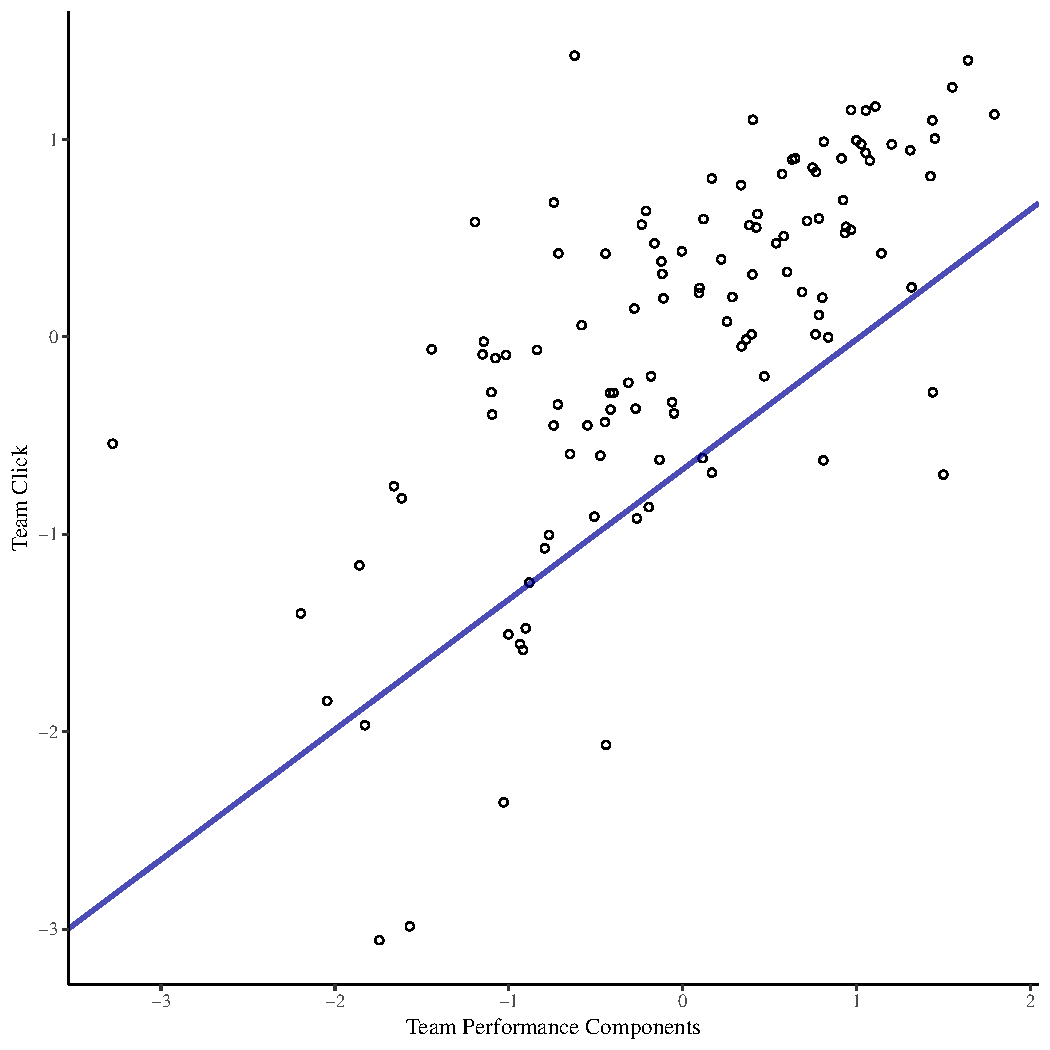
\includegraphics[scale = .5]{images/jasClickModelSlope}
  \caption{Team Performance Components predicts Team Click. Both variables are factors expressed as z-scores ($mean \approx 0, SD \approx 1$).  The line of best fit has been adjusted based on parameter estimates of the LMER ($n = 98$).}
  \label{fig:jasClickModelSLope}
\end{figure}



\myparagraph{Pre- to Post-Tournament}
Results of the Pre- to Post-Tournament data also supported predictions.  The model revealed a significant positive relationship between Team Performance Components Change and change in feelings of Team Click Change ($\beta = .52$ ($95\% CI =  .33, .71$), $SE = .09$, $t(11.07) = 5.47$, $p < .0001$, $marginal R^2 = .40$, $conditional R^2 = .47$).  No other main effects were significant (see Table ~\ref{tab:MLM21aJointActionSuccesscClick} in Appendix ~\ref{app8:tournamentSurvey} Section ~\ref{app8:211a} for results of all iterations of the model).  Model residuals were normally distributed around zero ($W = .98, p = .24$), and individual cases had low influence on the model (Cook's Distances all  $< .20 $, see Appendix ~\ref{app8:tournamentSurvey} Figure \ref{fig:MLM21aAssumptions}).

This model supported the prediction that positive change in perceptions of Team Performance Components are associated with increase in feelings of team click.  On average, Athletes who reported a positive increase in perceptions of components of team performance also reported a positive increase in feelings of team click throughout the Tournament.  The model-adjusted slope depicting the relationship between these two variables is included in Figure ~\ref{fig:jasClickDeltaModelSLope}.

\begin{figure}[htbp]
  \centering
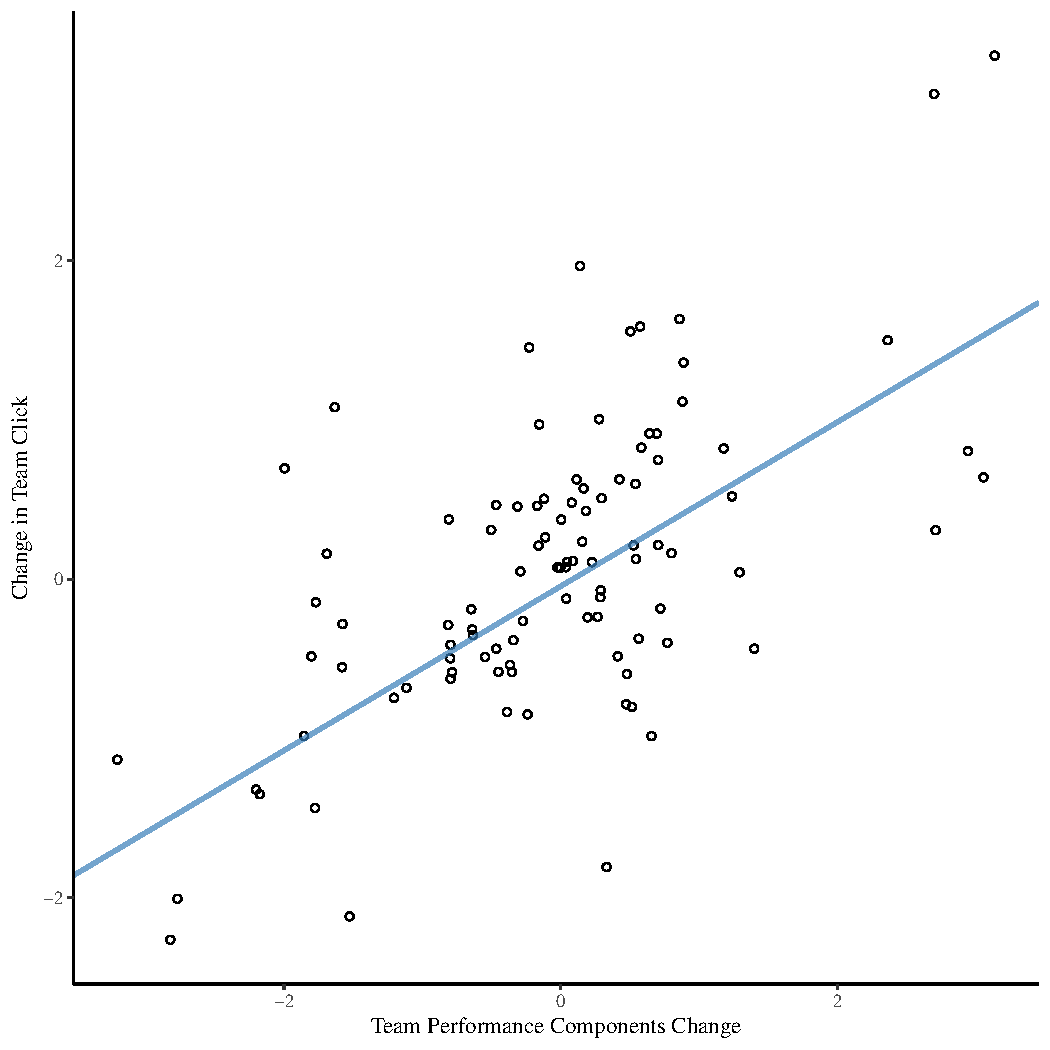
\includegraphics[scale=.5]{images/jasClickDeltaModelSlope}
  \caption{Team Performance Components Change predicts change in Team Click Change. The slope has been adjusted according to the parameter estimates of the linear model ($n = 97$).}
  \label{fig:jasClickDeltaModelSLope}
\end{figure}

In sum, results suggest more positive perceptions of technical components of team performance are associated with higher levels of Team Click. A positive increase in perceptions of Team Performance Components predicts a positive increase in feelings of Team Click between Pre- and Post-Tournament surveys, suggesting that athletes who perceived an increase in success of components of team performance also experienced an increase in feelings of team click. Together, these results support a relationship between joint action and team click.






\subsubsection{Prediction 1.b: Team Performance Vs Expectations predict Team Click}

\myparagraph{Post-Tournament}
Results of the model revealed a significant positive relationship between Team Performance Vs Expectations and Team Click, $\beta = .52$ ($95\% CI =  .28, .77$), $SE = .12$, $t(14.00) = 4.24$, $p < .0008$, $marginal R^2 = .40$, $conditional R^2 = .56$.  All other fixed effects did not significantly predict team click, but did improve the model fit, as indicated by the reduced AIC and increased marginal $R^2$ value (see Appendix Table ~\ref{tab:MLM1bteamExpectationsClick} for the various iterations of the model).

Model residuals were normally distributed around zero ($W = .98, p = .28$), and individual cases had low influence on the model (Cook's Distances all $< .2$, see Appendix ~\ref{app8:tournamentSurvey} Figure ~\ref{fig:MLM1bAssumptions}).  These results provide support for the prediction that more positive violations of expectations around team performance predict higher feelings of team click.  The relationship between Team Performance Vs Expectations and Team Click is represented in Figure ~\ref{fig:teamPerfClickModelSlope}.  Results support the prediction that more positive perceptions of team performance relative to prior expectations is associated with higher levels of team click.


  \begin{figure}[htbp]
    \centering
  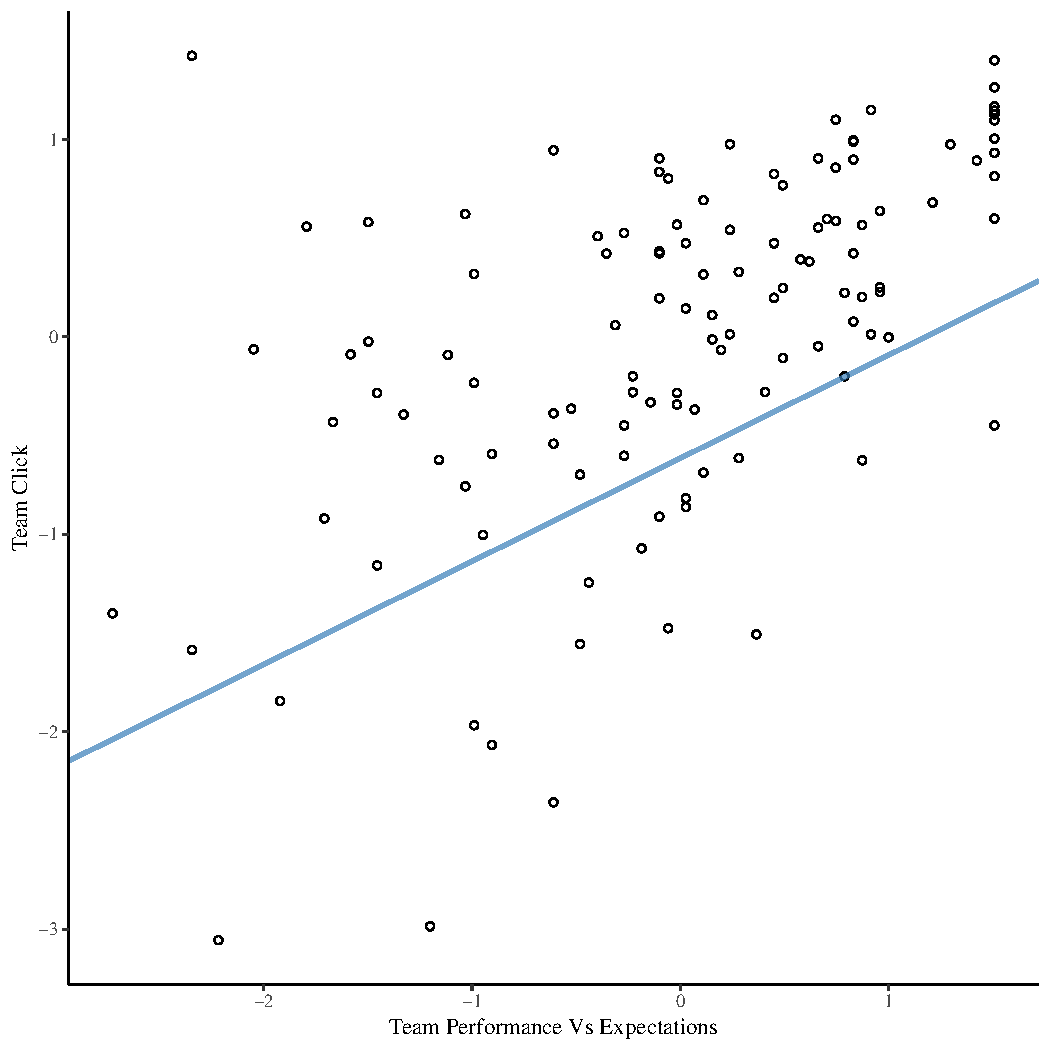
\includegraphics[scale=.5]{images/teamPerfClickModelSlope.pdf}
    \caption{Team Performance Vs Expectations predicts Team Click. The slope has been adjusted according to the predictions of the linear model ($n = 97$).}
    \label{fig:teamPerfClickModelSlope}
  \end{figure}



  \myparagraph{Pre- to Post-Tournament}
Given that the item measuring Athlete perceptions of overall team performance in the Pre-Tournament survey was not framed in terms of expectation violation (but instead in terms of more or less ``good'' or ``poor''), it was not possible to directly compare the Pre- and Post-Tournament measures.  Instead, the Post-Tournament measure of Team Performance Vs Expectation was used to predict change in feelings of team click between Pre- and Post-Tournament measurements.

The model revealed a significant positive relationship between Team Performance Vs Expectations and Team Click Change,  $\beta = .26$ ($95\% CI =  .03, .48$), $SE = .11$, $t(27.88) = 2.26$, $p = .03$, $marginal R^2 = .12$, $conditional R^2 = .22$, indicating that athletes who were more positive about their appraisals of team performance following the Tournament on average experienced an increase in feelings of team click.

Examination of model residuals revealed that they were not normally distributed around zero ($W = .96, p = .003$), due to positive skew ($.85$) (see Figure ~\ref{fig:MLM21bAssumptions} in Appendix ~\ref{app8:tournamentSurvey} Section ~\ref{app8:MLM21b}). Log-transformation of the outcome variable did not markedly improve the non-normality of residuals, ($Shapiro-Wilk = .96, p = .008$).    Instead, exclusion of outliers according to Tukey's method (observations above and below 1.5x the Inter Quartile Range (IQR), see \citep{Tukey1977}) improved the model fit such that residuals were normally distributed, ($Shapiro-Wilk = .99, p = .89$), and individual cases had low influence on the model (Cook's Distances all $< .10$, see Appendix Figure ~\ref{fig:MLM21bOutAssumptions}).\footnote{For a justification of transformation and exclusion methods, see Appendix ~\ref{app8:tournamentSurvey} Section ~\ref{app8:normality}.}

The adjusted model supported the original significant main effect of Team Performance Vs Expectations on Team Click Change, ($\beta = .36$ ($95\% CI =  .16, .55$), $SE = .10$, $t(9.78) = 3.66$, $p < .01$, $marginal R^2 = .16$, $conditional R^2 = .55$). The adjusted model also revealed a significant \textit{negative} main effect of Individual Performance Vs Expectations on Team Click Change (($\beta = -.19$ ($95\% CI =  -.03, -.35$), $SE = .10$, $t(91.90) = 2.26$, $p < .03$), such that more positive perceptions of individual performance relative to prior expectations predicted decrease in team click over the course of the Tournament.  All other main effects of the adjusted model were not significant (see Table ~\ref{tab:MLM21bOutLogComparison}  in Appendix ~\ref{app8:tournamentSurvey} Section ~\ref{app8:MLM21b} for a comparison of adjusted models.  The slope of the outlier-adjusted model is included in a graphical representation of the relationship, see Figure ~\ref{fig:teamPerfClickDeltaModelSlope}.

These results generally confirmed the prediction that on average, athletes who experience more positive violations around perceptions of team performance following the Tournament experienced more positive increases in Team Click. By contrast, Athletes who on average experienced more positive expectation violation in relation to \textit{individual} performance, by contrast, reported less increase in Team Click.


%The adjusted model also revealed a significant negative effect of violations of expectations around \textit{individual} performance on team click, $\beta = -.008 (95\% CI =  -.01, .001), SE = .004, t(91.79) = -2.28, p = .03$,  which could suggest that athletes who experienced more positive violations about their own performance did not feel the team click as strongly.

    
% Table created by stargazer v.5.2 by Marek Hlavac, Harvard University. E-mail: hlavac at fas.harvard.edu
% Date and time: Tue, Jun 27, 2017 - 09:21:13
\begin{table}[!htbp] \centering 
  \caption{M2.1b cTeamClick ~ cPerformanceExpectations} 
  \label{tab:MLM21bcTeamPerfExpcClick} 
\begin{tabular}{@{\extracolsep{5pt}}lccc} 
\\[-1.8ex]\hline 
\hline \\[-1.8ex] 
 & \multicolumn{3}{c}{\textit{Dependent variable:}} \\ 
\cline{2-4} 
\\[-1.8ex] & \multicolumn{3}{c}{cTeamClick} \\ 
\\[-1.8ex] & (1) & (2) & (3)\\ 
\hline \\[-1.8ex] 
 (constant) & 0.10 & $-$0.57 & $-$0.64 \\ 
  & (0.13) & (0.30) & (0.44) \\ 
  & & & \\ 
 cTeamPerformanceExpectations &  & 0.01$^{*}$ & 0.01$^{*}$ \\ 
  &  & (0.004) & (0.005) \\ 
  & & & \\ 
 cIndPerformanceExpectations &  &  & $-$0.003 \\ 
  &  &  & (0.004) \\ 
  & & & \\ 
 objectiveCompetence &  &  & $-$0.13 \\ 
  &  &  & (0.11) \\ 
  & & & \\ 
 subjectiveCompetence &  &  & $-$0.16 \\ 
  &  &  & (0.09) \\ 
  & & & \\ 
 finalRank &  &  & 0.02 \\ 
  &  &  & (0.06) \\ 
  & & & \\ 
 minutesTotal &  &  & 0.003 \\ 
  &  &  & (0.005) \\ 
  & & & \\ 
 pointsTotal &  &  & 0.003 \\ 
  &  &  & (0.01) \\ 
  & & & \\ 
\hline \\[-1.8ex] 
Marginal R-squared &  &  & .40 \\ 
Conditional R-squared &  &  & .47 \\ 
Observations & 99 & 99 & 97 \\ 
Log Likelihood & $-$130.59 & $-$127.00 & $-$123.15 \\ 
Akaike Inf. Crit. & 267.19 & 266.01 & 270.30 \\ 
Bayesian Inf. Crit. & 274.97 & 281.58 & 301.20 \\ 
\hline 
\hline \\[-1.8ex] 
\textit{Note:}  & \multicolumn{3}{r}{$^{*}$p$<$0.05; $^{**}$p$<$0.01; $^{***}$p$<$0.001} \\ 
\end{tabular} 
\end{table} 

    
\begin{table}
\begin{center}
\begin{tabular}{l c c c }
\toprule
 & Controls & Log-adjusted & Outliers removed \\
\midrule
(constant)                                 & $0.33$               & $\mathbf{1.27}^{***}$ & $0.40$                \\
                                           & $(0.51)$             & $(0.16)$              & $(0.39)$              \\
Team Performance Vs Expectations           & $\mathbf{0.30}^{**}$ & $\mathbf{0.09}^{*}$   & $\mathbf{0.32}^{***}$ \\
                                           & $(0.11)$             & $(0.04)$              & $(0.08)$              \\
Ind Performance Vs Expectations            & $-0.10$              & $-0.03$               & $\mathbf{-0.22}^{**}$ \\
                                           & $(0.10)$             & $(0.03)$              & $(0.08)$              \\
Objective Competence                       & $-0.15$              & $-0.05$               & $0.03$                \\
                                           & $(0.12)$             & $(0.04)$              & $(0.10)$              \\
Subjective Competence                      & $-0.15$              & $-0.05$               & $-0.03$               \\
                                           & $(0.09)$             & $(0.03)$              & $(0.08)$              \\
Final Rank                                 & $-0.01$              & $-0.00$               & $-0.08$               \\
                                           & $(0.06)$             & $(0.02)$              & $(0.04)$              \\
Minutes Total                              & $0.00$               & $0.00$                & $-0.00$               \\
                                           & $(0.01)$             & $(0.00)$              & $(0.00)$              \\
Points Total                               & $0.00$               & $0.00$                & $0.01$                \\
                                           & $(0.01)$             & $(0.00)$              & $(0.01)$              \\
Fatigue                                    & $-0.08$              & $-0.00$               & $-0.07$               \\
                                           & $(0.11)$             & $(0.04)$              & $(0.09)$              \\
Extraverted                                & $-0.06$              & $-0.02$               & $0.01$                \\
                                           & $(0.07)$             & $(0.02)$              & $(0.05)$              \\
\midrule
AIC                                        & 253.92               & 50.47                 & 200.30                \\
BIC                                        & 288.92               & 85.47                 & 234.66                \\
Log Likelihood                             & -112.96              & -11.23                & -86.15                \\
Num. obs.                                  & 90                   & 90                    & 86                    \\
Num. groups: team                          & 13                   & 13                    & 13                    \\

\bottomrule
\multicolumn{4}{l}{\scriptsize{Coefficients with $p < 0.05$ in \textbf{bold}. Effect size of model excluding outliers: Marginal $R^2 = .17$, Conditional $R^2 = .20$}}
\end{tabular}
\caption{Prediction 2: Team Click Change predicts Social Bonding Change in the Post-Tournament survey data (n = 90).}
\label{tab:MLM21bOutLogComparison}
\end{center}
\end{table}



    \begin{figure}[htbp]
      \centering
    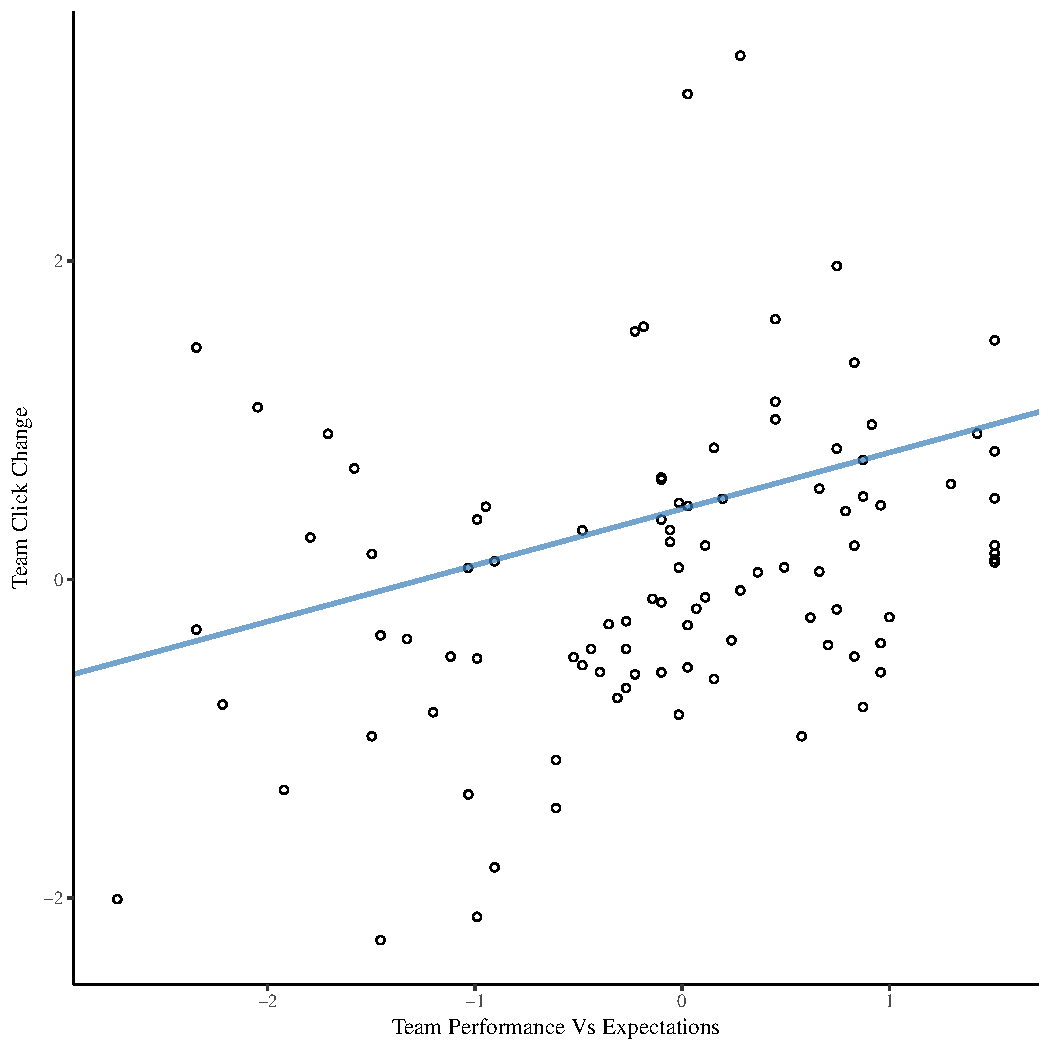
\includegraphics[scale=.5]{images/teamPerfClickDeltaModelSlope.pdf}
      \caption{Team Performance Vs Expectations predicts change in Team Click. The blue slope is the original line of best fit, the red slope has been adjusted according to the predictions of the linear model}
      \label{fig:teamPerfClickDeltaModelSlope}
    \end{figure}


  \myparagraph{Overall Tournament}
Analysis of the Overall Tournament subset confirmed the prediction.
The model revealed a significant relationship between Team Performance Vs Expectations  and Team Click, $\beta = .71$ ($95\% CI = .62, .80$), $SE = .001$, $t(193.20) = 16.29$, $p < .0001$, $marginal R^2 = .63$, $conditional R^2 = .69$.
The model also indicated that individual performance expectation violation significantly predicted team click, $\beta = .004$ ($95\% CI =  .04, .20$), $SE = .04$, $t(311.7) = 2.81$, $p < .01$, as did Subjective Competence, $\beta = .08$ ($95\% CI =  .002, .15$), $SE = .04$, $t(292) = 2.00$, $p = .02$  (see Table ~\ref{tab:MLM31ateamPerfClickTournament} for full description of results).  The relationship between Team Performance Vs Expectations  and Team Click is represented graphically in Figure ~\ref{fig:teamPerfClickOverallModelSlope}.

The residuals of the model were normally distributed around zero, ($W = .99, p = .11$), and individual cases had low influence on the model (Cook's Distances all $< .05$; see Appendix ~\ref{app8:tournamentSurvey} Figure ~\ref{fig:MLM31aAssumptions} for a full report of model assumptions).

Results of the model suggest that athletes whose expectations around team performance were more positively violated also experienced stronger feelings of team click.  The model also revealed main effects of Individual Performance Vs Expectation and Subjective Competence, adding further evidence to the possibility that perceptions of individual performance also play a role in producing perceptions of team click.   also appears that more positive expectations about individual performance, and higher levels of self-reported technical competence predicted higher levels of team click.


   \begin{figure}[htbp]
     \centering
   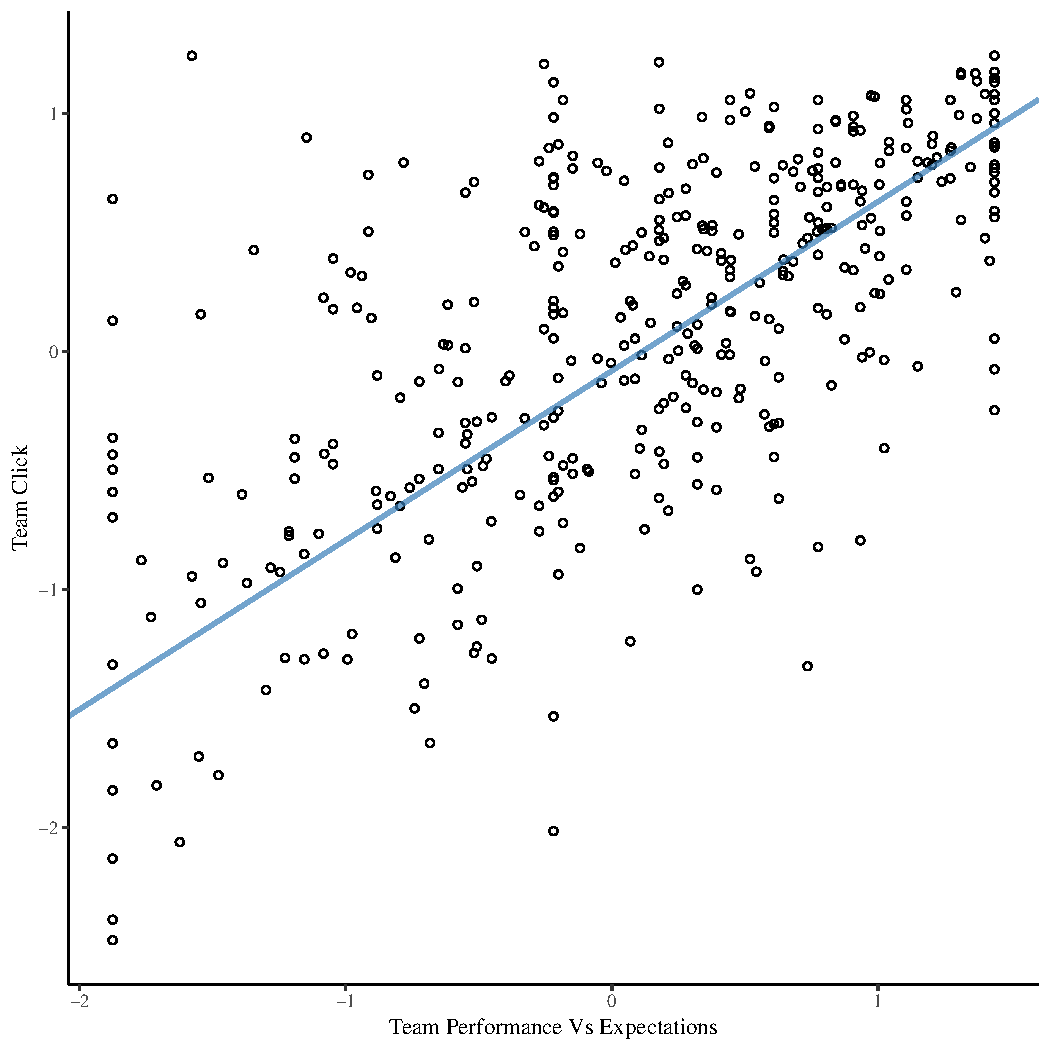
\includegraphics[scale=.5]{images/teamPerfClickOverallModelSlope.pdf}
     \caption{Team Performance Vs Expectations predicts Team Click in Overall Tournament subset.  The slope reflects the parameter estimates of the LMER model ($n = 331$).}
     \label{fig:teamPerfClickOverallModelSlope}
   \end{figure}



\myparagraph{Prediction 1.b: Summary of results}
Results from each subset supported the prediction that more positive expectation violation around team performance is associated with team click.  There was some evidence to suggest that individual performance violation may also predict team click, but results (from Pre- to Post Tournament data and the Overall Tournament data) were in
opposite directions.




\subsection{Prediction 1.c: Team Performance Components predicts Team Click, moderated by Team Performance Vs Expectations}

Did more positive violation of expectations surrounding team performance condition a direct relationship between perceptions of components of team performance and team click?  This prediction was tested in the Post-Tournament and Pre - to Post-Tournament data set.

  \subsubsection{Post-Tournament}
Team Performance Vs Expectations was added to the model as an interaction presented in Prediction 1.a. Results revealed that the interaction between Team Performance Components and Team Performance Vs Expectations was not significant, $\beta = .002$ ($95\% CI =  -.0062, .0063$), $SE = .08$, $t(39.7) = .026$, $p = .98$, $marginal R^2 = .56$, $conditional R^2 = .65$ (see Appendix ~\ref{app8:tournamentSurvey}, Table ~\ref{tab:MLM1cPerformanceClickInteraction}).  The inclusion of the interaction term failed to improve upon the fit of the previous model, judging by the relative goodness of fit, $AIC(1.c) = 217.91$ compared to $AIC(1.a) = 209.48$, $SD = .52 $, $\chi^2(18, N = 97) = 3.56$, $ p =.74$.

\subsubsection{Pre- to Post-Tournament}
The interaction effect of Team Performance Vs Expectations and Team Performance Components on Team Click Change was not significant, $\beta = .004$ ($95\% CI =  -.002, .01$), $SE = .003$, $t(30.14) = 1.42$, $p = .17$, and failed to improve the model fit, $\chi^2 = 2.72$, $ p = .44$ (see Table ~\ref{tab:MLM21ccTeamPerfExpcClickInt}).  This result suggests that perceptions of team performance relative to prior expectations did not have an additive effect on the positive relationship between perceptions of Team Performance Components and Team Click.

\myparagraph{Prediction 1.c: Summary of results}
Results did not offer support for the prediction for an interaction effect of Team Performance Components and Team Performance Vs Expectations on team click.






\subsection{Prediction 2: Team Click predicts Social Bonding}


\myparagraph{Post-Tournament}
 Results supported the prediction.  A LMER model revealed a significant relationship between Team Click and Social Bonding, $\beta = .67$ ($95\% CI =  .51, .83$), $SE = .08$, $t(15.23) = 8.22$, $p < .0001$, $marginal R^2 = .49$, $conditional R^2 = .51$ (see Table ~\ref{tab:MLM2aTeamClickBonding} in Appendix ~\ref{chap:tournamentSurvey} Section ~\ref{app8:MLM2a} for a full description of results).  Model residuals were normally distributed around zero ($W = .98, p = .14$), and individual cases had low influence on the model (Cook's Distances all $< .15$, see Appendix ~\ref{app8:tournamentSurvey} Figure ~\ref{fig:MLM2aAssumptions} for a full report of model assumptions).  The model supported the prediction that higher levels of team click are associated with higher levels of social bonding.  The relationship between these two variables is represented graphically in Figure ~\ref{fig:clickBondModelSlope}).

  \begin{figure}[htbp]
    \centering
  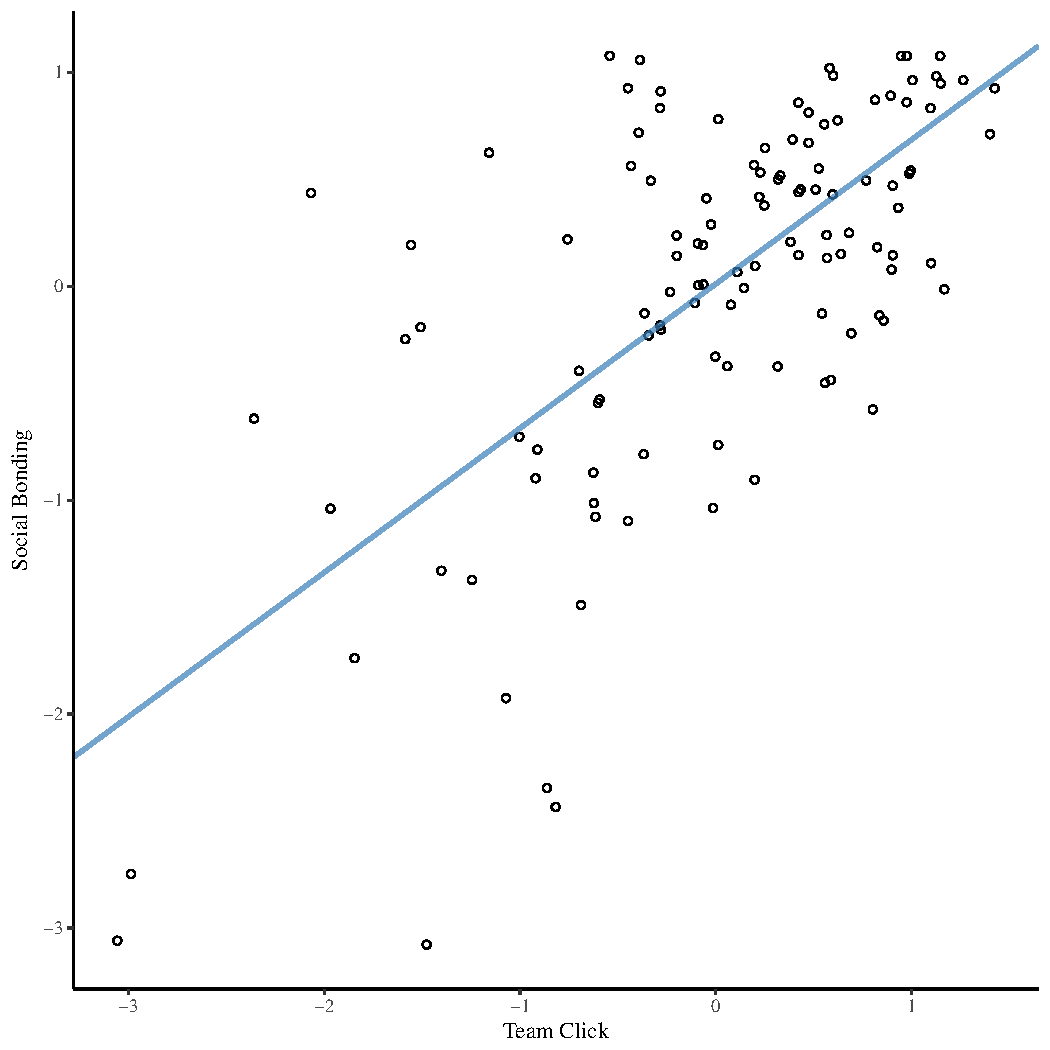
\includegraphics[scale=.5]{images/clickBondModelSlope.pdf}
    \caption{Team Click predicts Social Bonding in Post-Tournament survey data. The slope reflects the model parameter estimates of the LMER ($n = 97$).}
    \label{fig:clickBondModelSlope}
  \end{figure}



  \myparagraph{Pre- to Post-Tournament}
Results of the Pre- to Post survey data also supported the prediction.
The LMER model revealed a significant positive effect of Team Cick Change on Social Bonding Change, ($\beta = .40$ ($95\% CI =  .16, .64$), $SE = .12$, $t(7.02) = 3.31$, $p = .01$, $marginal R^2 = .17$, $conditional R^2 = .23$; see Table ~\ref{tab:MLM22acClickcBonding} in Appendix ~\ref{chap:tournamentSurvey} Section ~\ref{app8:MLM2a} for a full description of model estimates).  Model residuals were normally distributed around zero ($Shapiro-Wilk = .98, p = .15$). and individual cases had low influence on the model (Cook's Distances all $< .6$, see Appendix ~\ref{chap:tournamentSurvey} Section ~\ref{app8:MLM2a} Figure ~\ref{fig:MLM22aAssumptions} for model assumptions).  This model suggests that athletes who experienced an increase in feelings of team click also experienced an increase in feelings of social bonding towards their team.
Figure ~\ref{fig:clickBondDeltaModelSlope} depicts the relationship between Team Click Change and Social Bonding Change.

  \begin{figure}[htbp]
    \centering
  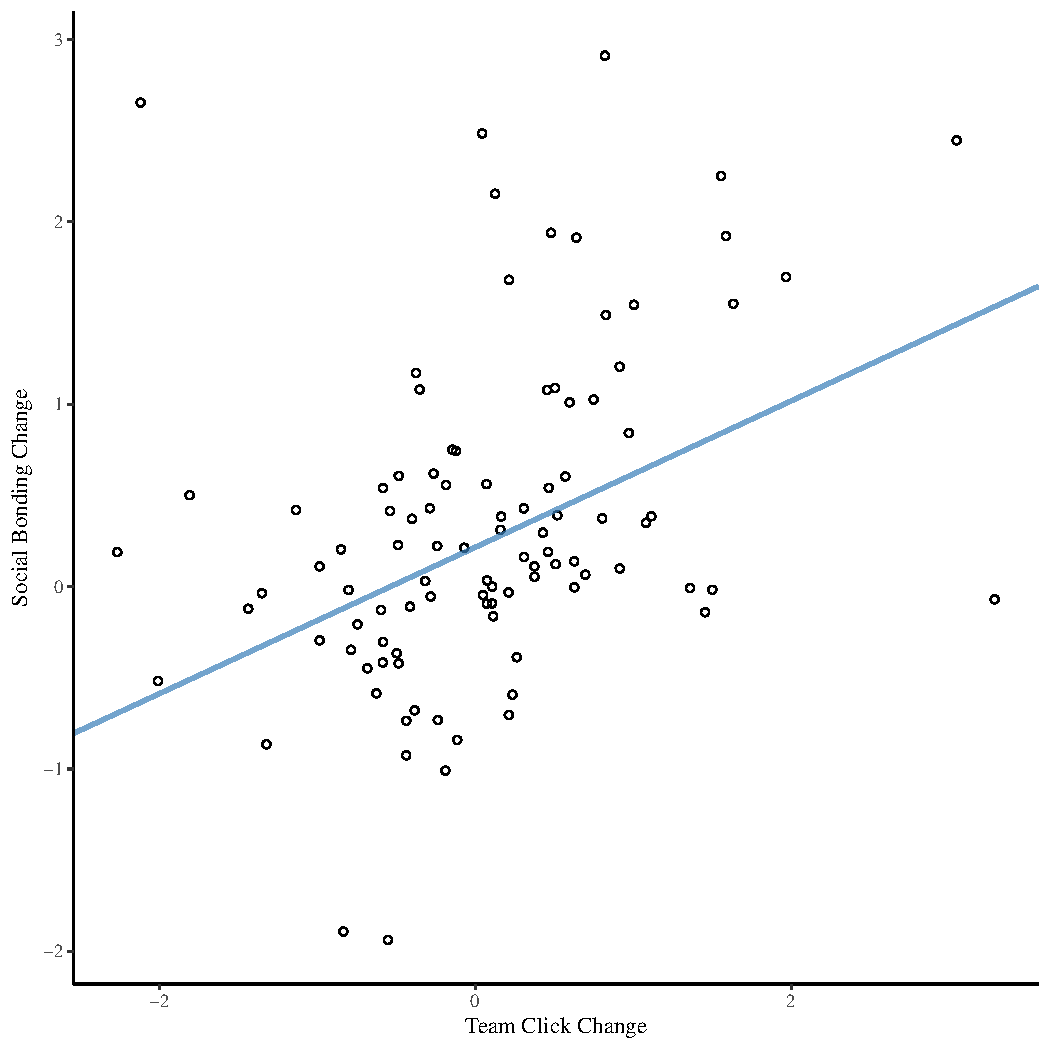
\includegraphics[scale=.5]{images/clickBondDeltaModelSlope.pdf}
    \caption{Change in Team Click predicts change in Social Bonding in the Pre- to Post-Tournament subset of survey data. The slope reflects parameter estimates of the LMER ($n = 97$).}
    \label{fig:clickBondDeltaModelSlope}
  \end{figure}


\myparagraph{Overall Tournament}
A model of the Overall Tournament data also supported the prediction. The LMER revealed a significant positive relationship between  Team Click and Social Bonding, $\beta = .64$ ($95\% CI = .55, .74$), $SE = .05$, $t(87.4) = 13.84$, $p < .0001$, $marginal R^2 = .49$, $conditional R^2 = .66$ (see Table ~\ref{tab:MLM31bclickBondingTournament} in Appendix ~\ref{chap:tournamentSurvey} Section ~\ref{app8:MLM32a} for complete description of model comparisons and estimates).

Model residuals were not normally distributed around zero, ($W = .92, p < .00001$), owing to high negative skew ($-1.24$) and high kurtosis (5.12) (see Appendix ~\ref{app8:tournamentSurvey} Figure ~\ref{fig:MLM31bAssumptions}). Both log transformation ($W = .92, p < .00001$) and outlier removal ($W = .96, p < .00001$) procedures improved the model fit only marginally (not within the accepted bounds of normality).

To resolve this assumption violation, the outcome variable was first subjected to outlier-removal, and then subsequently log-transformed, which appeared to improve the distribution of residuals somewhat, ($W = .98, p = .0002$, see Table ~\ref{MLM31bclickBondingTournamentModelComparison} for adjusted model comparisons and Appendix Figure ~\ref{fig:MLM31bLogOutAssumptions} for adjusted model residuals).  The failure of this model to converge indicated that it was not a robust reflection of the Overall Tournament data.











\subsection{Prediction 3: More positive perceptions of joint action success will predict higher levels of social bonding}



\subsubsection{Prediction 3.a: More positive perceptions of technical components of team performance will predict higher levels of social bonding }


\myparagraph{Post-Tournament}
The model revealed a significant effect of Team Performance Components on Social Bonding, $\beta = .45$ ($95\% CI =  .17, .73$), $SE = .14$, $t(23.4) = 3.19$, $p < .01$, $marginal R^2 = .27$, $conditional R^2 = .42$.  The model also revealed a significant positive effect of subjective measures of competence on Social Bonding, $\beta = .18$ ($95\% CI =  .03, .35$), $SE = .08$, $t(90.62) = 2.26$, $p = .03$ (full results in Table ~\ref{tab:MLM3aJointActionSuccessBonding}).

Model residuals were non-normally distributed ($W = .95, p = .0007$), owing to relatively large negative skew (-.87) (see Appendix Figure ~\ref{fig:MLM3aAssumptions}).  Analysis of the graphic relationship between Team Performance Components on Social Bonding indicated possibility of outliers biasing the model (see Figure ~\ref{fig:jasBondModelSlope}).  Exclusion of outliers appeared to improve the model fit, $\beta = .26$ ($95\% CI =  .05, .47$), $SE = .004$, $t(9.78) = 3.66$, $p < .01$, $marginal R^2 = .18$, $conditional R^2 = .34$.  The distribution of model residuals appeared to improve, but still violated the assumption of normality ($Shapiro-Wilk = .96, p = .009$).  Individual cases had low influence on the model (Cook's Distances all < .10).

Due to the \textit{positive} skew of the model residuals, the outcome variable was transformed by taking the log of the reversed scores of the outcome variable, i.e. $log10(k - y)$, where $k$ is a constant value from which each score for $y$ is subtracted so that the distribution of the outcome variable is reversed\citep{Howell2012}.
  \footnote{Reversing the distribution of the outcome variable allows the logarithmic function to normalise the distribution of the variable, by pushing them from the left hand side of the distribution towards the centre}
Transformed values were then returned to their original direction for analysis \citep{Field2012}.  Rebuilding the model with a log-transformed outcome variable appeared to improve the fit of the model more than the outlier-removed model, and avoided the removal of any observations.

Th is combination of adjustments achieved normal distribution of residuals ($W = .98, p = .08$), and the R-squared values for the model improved, $marginal R^2 = .27$, $conditional R^2 = .43$ (see Table ~\ref{tab:MLM3aJointActionSuccessBonding} for results of all three models, and Appendix ~\ref{app8:tournamentSurvey} Figures ~\ref{fig:MLM3aAssumptions}\nobreakdash~\ref{fig:MLM3aLogAssumptions}).Results of the log-transformed model were taken as satisfactory evidence for a significant positive relationship between perceptions of Team Performance Components and feelings of Social Bonding.
%While Levene's Test for Equality of Variance indicated that the assumption of homoscedasticity was met at the group-level, $F(13,83) = .80, p = .66$,

  \begin{figure}[htbp]
    \centering
  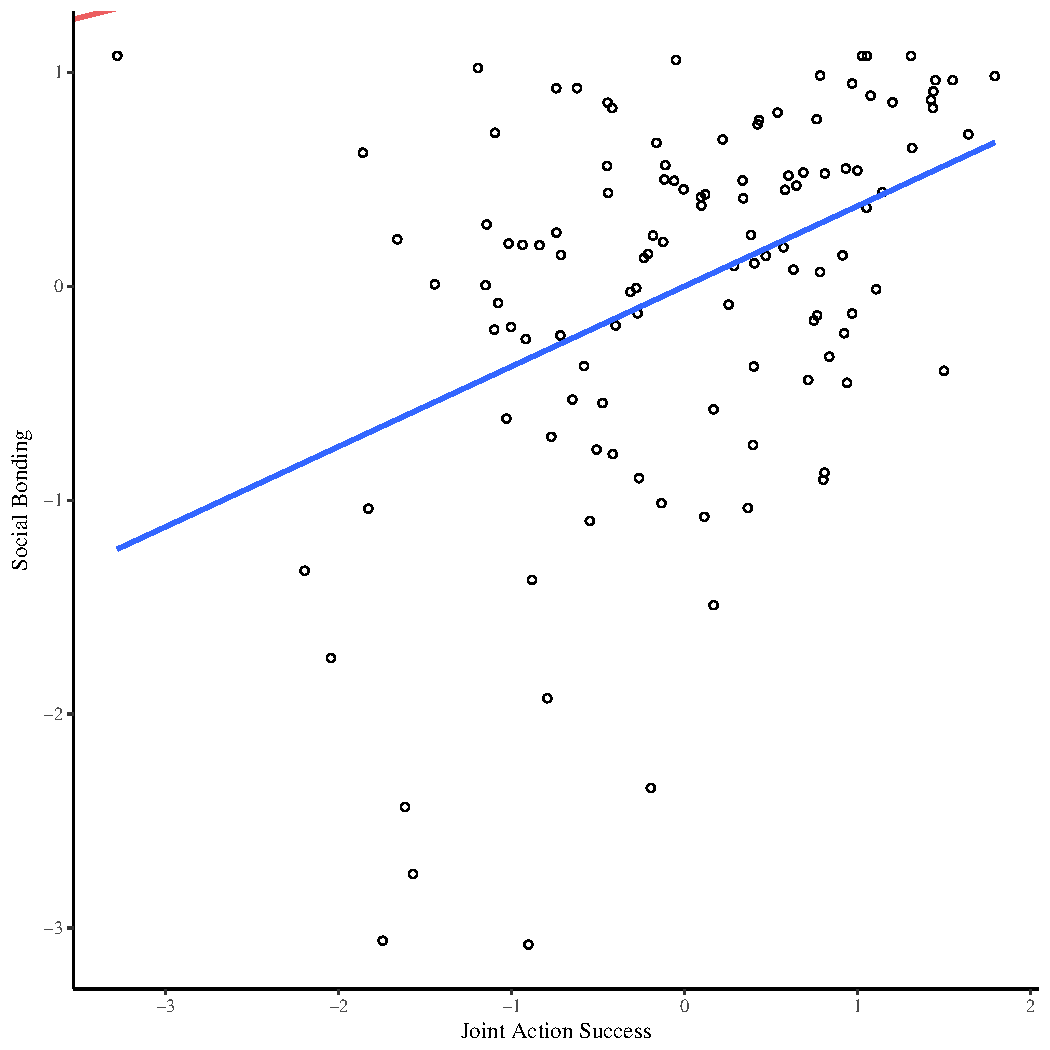
\includegraphics[scale=.5]{images/jasBondModelSlope.pdf}
    \caption{Team Performance Components predicts Social Bonding in Post-Tournament survey data. The line of best fit reflects the log-adjusted LMER model ($n = 97$).}
    \label{fig:jasBondModelSlope}
  \end{figure}




\myparagraph{Pre- to Post-Tournament}
Results of a LMER model revealed a significant positive effect of  Team Performance Components Change Social Bonding Change ($\beta = .38$ ($95\% CI =  .21, .56$), $SE = .09$, $t(97) = 4.26$, $p < .0001$, $marginal R^2 = .18$, $conditional R^2 = .18$), suggesting that on average, athletes who experienced an increase in positive perceptions of Team Performance Components as a result of the Tournament also experienced an increase in feelings of Social Bonding.  Notably, the model also revealed a significant \textit{negative} effect of perceptions of success in individual component performance and social bonding, $\beta = -.23$ ($95\% CI =  -.44, -.02$), $SE = .11$, $t(97) = -2.12$, $p = .04$, indicating that athletes whose attitudes towards their own performance increased in positivity showed an average decrease in feelings of social bonding between Pre- and Post-Tournament measures.
All other fixed effects were not significant, see Table ~\ref{tab:MLM23acJointActionSuccesscBonding}. Model residuals were normally distributed around zero ($W = .98, p = .19$), and individual cases had low influence on the model (Cook's Distances all $< .5$; see Figure ~\ref{fig:MLM23aAssumptions} in Appendix ~\ref{app8:tournamentSurvey} Section ~\ref{app8:MLM23a} for a full description of model assumptions).  See Figure ~\ref{fig:jasBondDeltaModelSlope} for a graphical representation of the relationship between Team Component Performance Change and Social Bonding Change.

This model supported the prediction that more positive perceptions perception of components of team performance significantly predict  higher levels of social bonding. The adjusted line of best fit generated by the model parameters is included in the scatterplot for comparison .


  \begin{figure}[htbp]
    \centering
  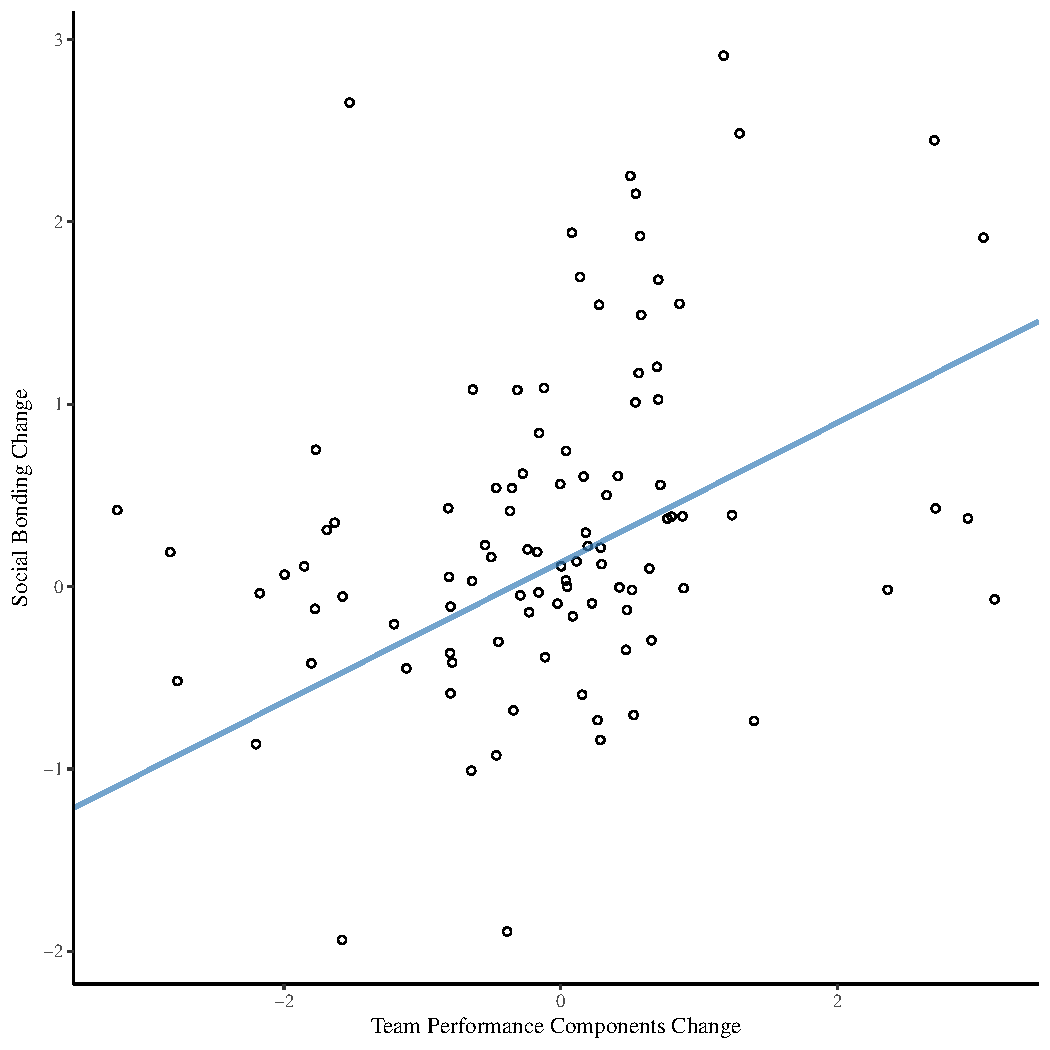
\includegraphics[scale=.5]{images/jasBondDeltaModelSlope.pdf}
    \caption{Team Performance Components Change predicts Social Bonding Change in Pre- to Post-Tournament survey data. The line of best fit reflects the parameter estimates of the LMER ($n = 97$).}
    \label{fig:jasBondDeltaModelSlope}
  \end{figure}




%  3) more positive perceptions of joint action success will predict higher levels of social bonding, driven by more positive 3.a) perceptions of components of team performance, or 3.b) violation of team performance expectations, or 3.b) an interaction between the two predictors.









\subsubsection{Prediction 3.b: More positive violations of team performance expectations predicts higher social bonding}
The model revealed a significant positive relationship between Team Performance Vs Expectations and Social Bonding, $\beta = .35$ ($95\% CI = .06, .64$), $SE = .14$, $t(12.80) = 2.39$, $p = .03$, $marginal R^2 = .20$, $conditional R^2 = .40$.  The model also revealed a significant positive effect of Subjective Competence on Social Bonding, $\beta = .19$ ($95\% CI =  .02, .36$), $SE = .08$, $t(90.37) = 2.24$, $p = .03$, such that athletes who provided higher ratings of their own technical competence in rugby (measured before the Tournament) reported higher levels of social bonding.

Model residuals were not normally distributed, ($W = .91, p < .0001$), owing to large negative skew ($-1.33$) and high kurtosis ($.49$). Re-running the model with a log-transformed outcome variable appeared to make the best improvement to model residuals more than the outlier-removed model (see Appendix ~\ref{app8:tournamentSurvey} Section ~\ref{app8:MLM3b} Table ~\ref{tab:MLM3bExpectationsBonding}). In the log-transformed model, the distribution of model residuals appeared most normal,  ($W = .97, p = .04$), and the R-squared values for the model improved, $marginal R^2 = .23$, $conditional R^2 = .44$.
Individual cases had low influence on the model (Cook's Distances all $< .15$, see Appendix ~\ref{app8:tournamentSurvey} Section ~\ref{app8:MLM3b} Figures ~\ref{fig:MLM3bAssumptions} and ~\ref{fig:MLM3bLogAssumptions} for a comparison of model assumptions between the original and log-transformed model).
Owing to non-normally distributed residuals, this model does not provide robust support for the prediction that team performance expectation violations relates directly to social bonding.



  \myparagraph{Pre- to Post-Tournament}
  %\subsubsection{2.3.b $\Delta$Social Bonding $\sim$ Team Performance Vs Expectations}
  A model revealed a marginally significant main effect of Team Performance Vs Expectations on Social Bonding Change $\beta = .20$ ($95\% CI =  -.0004, .02$), $SE = .11$, $t(97) = 1.87$, $p = .07$, $marginal R^2 = .05$, $conditional R^2 = .05$.  Examination of model residuals revealed that they were not normally distributed around zero ($Shapiro-Wilk = .96, p = .008$).  Re-running the model with a log-transformed outcome variable and outliers excluded improved the normality of residuals, ($Shapiro-Wilk = .98, p = .24$).
  However the effect of Team Performance Vs Expectations on Social Bonding was no longer significant, $\beta = .04$ ($95\% CI =  .02, .10$), $SE = .03$, $t()) = 1.29$, $p = .01$, $marginal R^2 = .03$, $conditional R^2 = .09$ (see Table ~\ref{tab:MLM23bcBondingteamPerfExp} in Appendix ~\ref{app8:tournamentSurvey} Section ~\ref{app8:MLM23b} for full description of results).

  These results suggest that perceptions of team relative to prior expectations between Pre- and Post-Tournament measurements did not suitably explain observed variation in Social Bonding Change.





  \myparagraph{Overall Tournament}
  The initial model failed to converge with the random slope and intercept model structure.  As such, the model was simplified to estimate only the random slope. This simplified model revealed a significant positive relationship between Team Performance Vs Expectations and Social Bonding, $\beta = .46$ ($95\% CI =  .35, .57$), $SE = .05$, $t(331.00) = 8.48$, $p < .0001$, $marginal R^2 = .40$, $conditional R^2 = .40$.

  The model also revealed a significant relationship between Individual Performance Vs Expectations and Social Bonding, $\beta = .005$ ($95\% CI =  .002, .009$), $SE = .002$, $t(303.4) = 2.80$, $p < .01$, as well as subjective competence and social bonding, $\beta = .01$ ($95\% CI =  .01, .18$), $SE = .04$, $t(265.3) = 2.24$, $p = .03$ (see Table ~\ref{tab:MLM32ateamPerfBondingTournament} in Appendix ~\ref{app8:tournamentSurvey} Section ~\ref{app8:MLM32a}for full description of model estimates).  Model residuals were non-normally distributed, ($W = .97, p < .00001$), with negative skew ($-.6$), and higher than normal kurtosis, see Appendix ~\ref{app8:tournamentSurvey} Figure ~\ref{fig:MLM32aAssumptions}.  A model in which the outcome was log-transformed following removal of outliers provided the best possible fit for the available data ~\ref{MLM32ateamPerfBondingTournamentModelComparison}. While the distribution of errors was still non-normal, ($W = .99, p = .03$),  error terms appear much more evenly distributed around zero than the original model, albeit with a slight negative skew ($-.1$).
  The adjusted model provided confirmation that the significant positive effect of team performance expectation violation on Social Bonding,  $\beta = .16$ ($95\% CI =  .12, .20$), $SE = .02$, $t(336.80) = 7.98$, $p < .0001$, $marginal R^2 = .36$, $conditional R^2 = .36$.

   
\begin{table}
\begin{center}
\begin{tabular}{l c c c c }
\toprule
 & Main effect & Controls & Log-transformed & Log and outliers \\
\midrule
(constant)                        & $-0.00$               & $\mathbf{0.51}^{*}$   & $\mathbf{1.71}^{***}$ & $\mathbf{1.64}^{***}$ \\
                                  & $(0.04)$              & $(0.26)$              & $(0.06)$              & $(0.08)$              \\
Team Performance Vs Expectations  & $\mathbf{0.59}^{***}$ & $\mathbf{0.47}^{***}$ & $\mathbf{0.11}^{***}$ & $\mathbf{0.07}^{***}$ \\
                                  & $(0.04)$              & $(0.06)$              & $(0.01)$              & $(0.02)$              \\
Ind Performance Vs Expectations   &                       & $\mathbf{0.25}^{***}$ & $\mathbf{0.05}^{***}$ & $0.01$                \\
                                  &                       & $(0.06)$              & $(0.01)$              & $(0.02)$              \\
Objective Competence              &                       & $0.07$                & $0.02$                & $0.01$                \\
                                  &                       & $(0.05)$              & $(0.01)$              & $(0.02)$              \\
Subjective Competence             &                       & $0.09$                & $\mathbf{0.02}^{*}$   & $\mathbf{0.03}^{*}$   \\
                                  &                       & $(0.05)$              & $(0.01)$              & $(0.01)$              \\
Final Rank                        &                       & $-0.03$               & $-0.01$               & $-0.01$               \\
                                  &                       & $(0.02)$              & $(0.01)$              & $(0.01)$              \\
Minutes Total                   &                       & $-0.01$  & $-0.00$  & $-0.00$               \\
                                  &                       & $(0.00)$              & $(0.00)$              & $(0.00)$              \\
Points Total                      &                       & $0.00$                & $0.00$                & $0.00$                \\
                                  &                       & $(0.00)$              & $(0.00)$              & $(0.00)$              \\
Fatigue                           &                       & $0.00$                & $0.00$                & $0.00$                \\
                                  &                       & $(0.00)$              & $(0.00)$              & $(0.00)$              \\
Extraverted                       &                       & $-0.04$               & $-0.01$               & $-0.02$               \\
                                  &                       & $(0.03)$              & $(0.01)$              & $(0.01)$              \\
\midrule
AIC                               & 1083.79               & 752.42                & -131.94               & -8.28                 \\
BIC                               & 1104.27               & 800.83                & -83.53                & 38.54                 \\
Log Likelihood                    & -536.89               & -363.21               & 78.97                 & 17.14                 \\
Num. obs.                         & 444                   & 306                   & 306                   & 271                   \\
\bottomrule
\multicolumn{5}{l}{\scriptsize{Coefficients with $p < 0.05$ in \textbf{bold}. Effect sizes of the Log and outlier model: Marginal $R^2 = .36$, Conditional $R^2 = .36$}}
\end{tabular}
\caption{Prediction 3: Team Performance Vs Expectations predicts Social Bonding in the Overall Tournament survey data (n = 90).}
\label{tab:MLM32ateamPerfBondingTournament}
\end{center}
\end{table}


   
% Table created by stargazer v.5.2 by Marek Hlavac, Harvard University. E-mail: hlavac at fas.harvard.edu
% Date and time: Thu, Sep 14, 2017 - 09:42:11
\begin{table}[!htbp] \centering 
  \caption{Model Comparison: M3.2a socialBondingTournament ~ teamPerformanceExpectationsTournament} 
  \label{tab:MLM32ateamPerfBondingTournamentModelComparison} 
\scriptsize 
\begin{tabular}{@{\extracolsep{5pt}}lccc} 
\\[-1.8ex]\hline 
\hline \\[-1.8ex] 
 & \multicolumn{3}{c}{\textit{Dependent variable:}} \\ 
\cline{2-4} 
 & model & log-transformed & outliers+log-transformed \\ 
\\[-1.8ex] & (1) & (2) & (3)\\ 
\hline \\[-1.8ex] 
 (constant) & $-$0.70$^{***}$ & 1.42$^{***}$ & 1.42$^{***}$ \\ 
  & (0.18) & (0.04) & (0.06) \\ 
  & & & \\ 
 teamPerformanceExpectations & 0.01$^{***}$ & 0.003$^{***}$ & 0.003$^{***}$ \\ 
  & (0.002) & (0.0005) & (0.001) \\ 
  & & & \\ 
 indPerformanceExpectations & 0.01$^{**}$ & 0.001$^{**}$ & 0.0001 \\ 
  & (0.002) & (0.0004) & (0.001) \\ 
  & & & \\ 
 objectiveCompetence & 0.04 & 0.01 & 0.01 \\ 
  & (0.05) & (0.01) & (0.02) \\ 
  & & & \\ 
 subjectiveCompetence & 0.10$^{*}$ & 0.03$^{*}$ & 0.03$^{*}$ \\ 
  & (0.04) & (0.01) & (0.01) \\ 
  & & & \\ 
 finalRank & $-$0.04 & $-$0.01 & $-$0.01 \\ 
  & (0.02) & (0.005) & (0.01) \\ 
  & & & \\ 
 minutesTotal & $-$0.003 & $-$0.001 & $-$0.001 \\ 
  & (0.002) & (0.001) & (0.001) \\ 
  & & & \\ 
 pointsTotal & 0.001 & 0.0001 & 0.0000 \\ 
  & (0.004) & (0.001) & (0.001) \\ 
  & & & \\ 
\hline \\[-1.8ex] 
Marginal R-squared & .33 & .11 & .09 \\ 
Conditional R-squared & .53 & .23 & .17 \\ 
Shapiro-Wilk Test (p-value) & .97($<$.00001) & .96($<$.00001) & .97($<$.00001) \\ 
Observations & 331 & 331 & 294 \\ 
Log Likelihood & $-$373.85 & 96.45 & 21.56 \\ 
Akaike Inf. Crit. & 777.70 & $-$162.91 & $-$13.13 \\ 
Bayesian Inf. Crit. & 834.73 & $-$105.88 & 42.13 \\ 
\hline 
\hline \\[-1.8ex] 
\textit{Note:}  & \multicolumn{3}{r}{$^{*}$p$<$0.05; $^{**}$p$<$0.01; $^{***}$p$<$0.001} \\ 
\end{tabular} 
\end{table} 



   \begin{figure}[htbp]
     \centering
   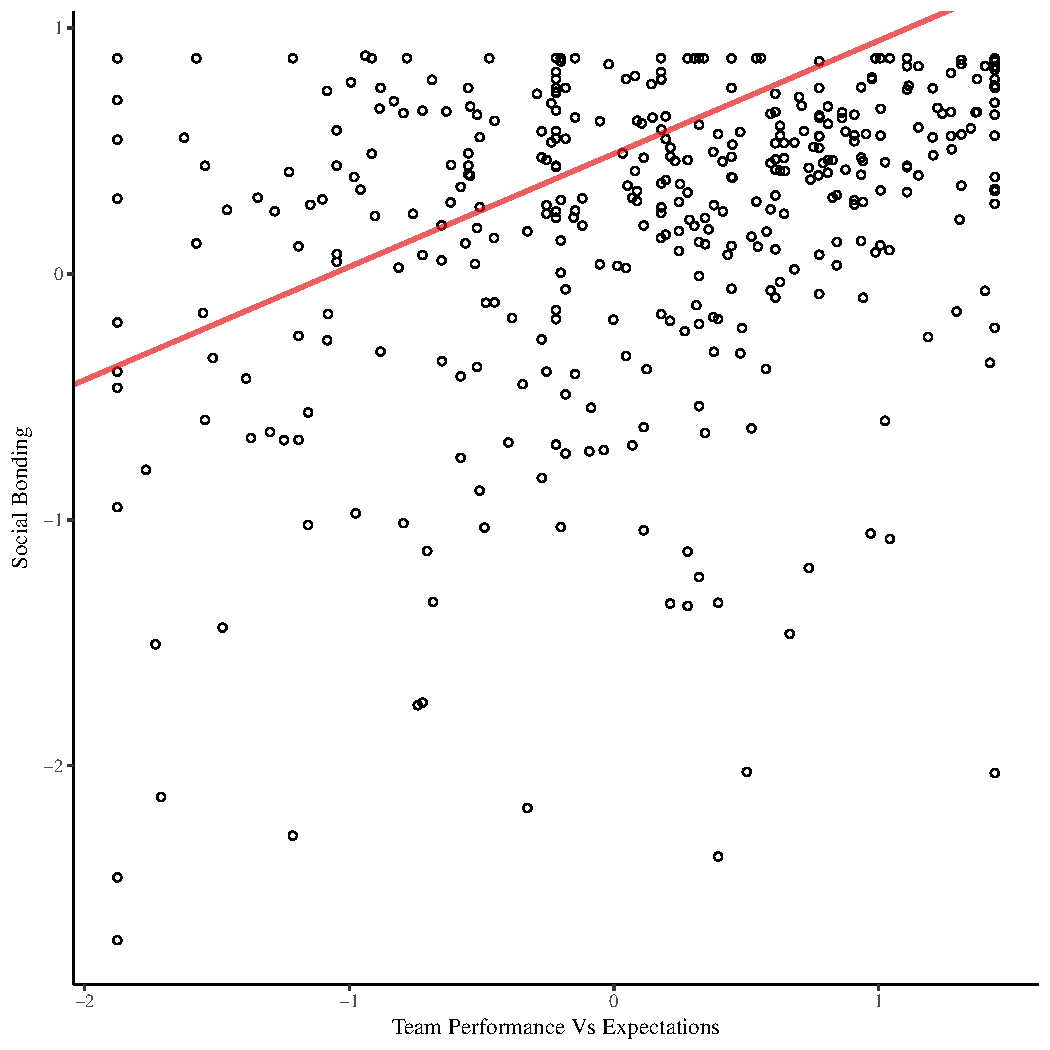
\includegraphics[scale=.5]{images/teamPerfBondOverallModelSlope.pdf}
     \caption{Team Performance Components predicts Social Bonding in Post-Tournament survey data. The blue slope is the original line of best fit, the red slope has been adjusted according to the predictions of the linear model.}
     \label{fig:teamPerfBondOverallModelSlope}
   \end{figure}



\subsection{Prediction 4: Feelings of team click mediate the relationship between perceptions of success in joint action and feelings of social bonding}

  \subsubsection{4.a: Team Click mediates the relationship between Team Performance Components and Social Bonding}

  \myparagraph{Post-Tournament}
  Mediation analyses were conducted using linear mixed effects regressions in the Causal Mediation Analysis package in R (Version 4.4.5).  To make inferences concerning the average indirect and total effects, quasi-Bayesian Markov Chain Monte Carlo (MCMC) method based on normal approximation and 1000 simulations was used to estimate the 95\% Confidence Intervals \citep{Tofighi2016a,Imai2010}. MCMC estimation is a form of non-parametric bootstrapping whereby the sampling distribution for the effect of interest is not assumed to be normal but is instead simulated from the model estimates and their asymptotic variances and covariances \cite{Preacher2008}.

  Results of the mediation analysis revealed significant average indirect effect of Team Performance Components on Social Bonding attributable to Team Click, $\beta = .37, 95\% CI = .20 , .59, p < .001$.  When controlling for the effect of team click on Social Bonding, the average direct effect between Team Performance Components and Social Bonding was no longer significant, $\beta = -.006, 95\% CI = -.27 , .23, p = .96 $ (see Figure ~\ref{fig:MLM4aMediationAnalysis}). The direct effect diminished such that including Team Performance Components in the model produced a total effect that was marginally \textit{smaller} than the indirect effect alone, $\beta = .36, 95\% CI = .13 , .61, p = .01$. These results suggest that feelings of team click fully mediate the relationship between perceptions of Team Performance Components and social bonding.


  %Residuals of the mediation model were normally distributed around zero, ($W = .99, p < .28$, see Figure ~\ref{fig:MLM4aAssumptions} for model assumptions).

  \begin{figure}[htbp]
    \centering
    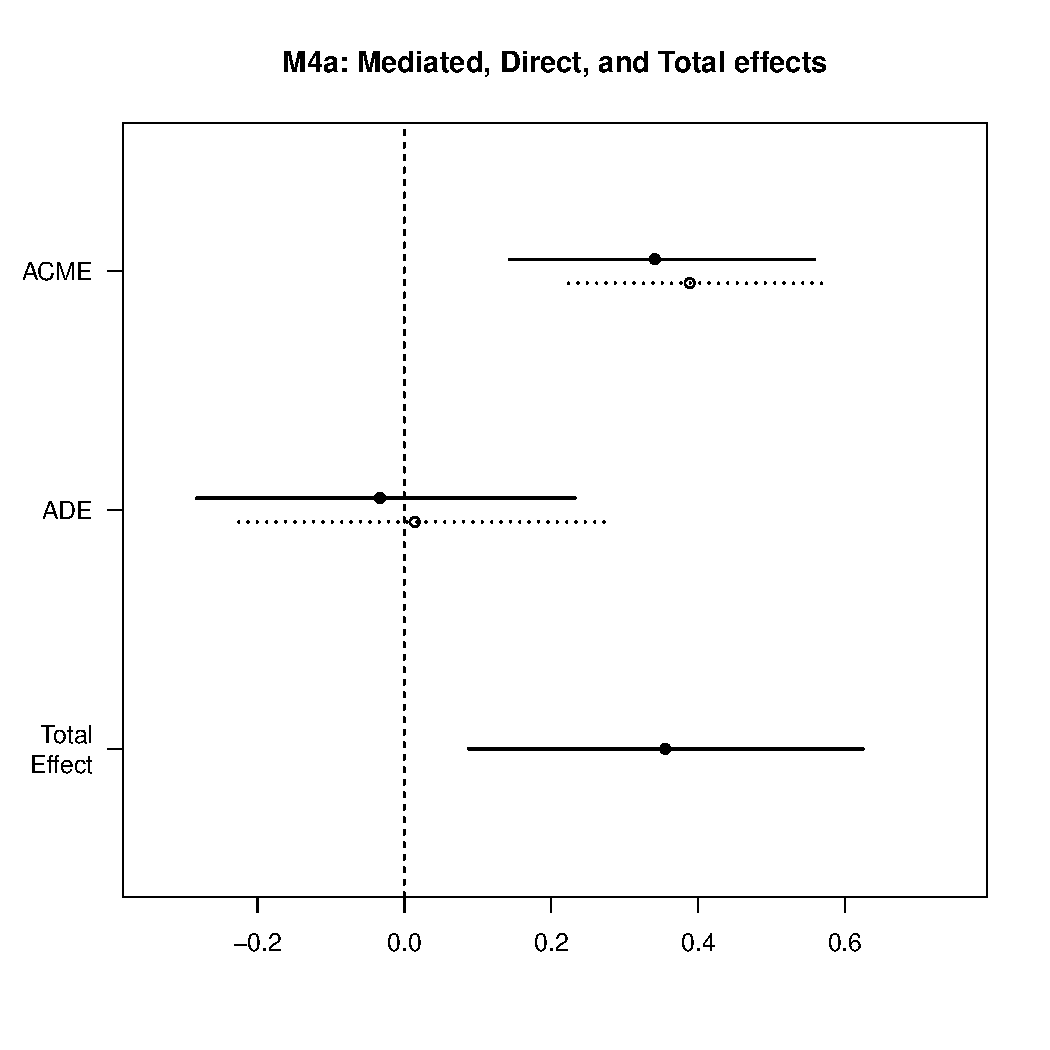
\includegraphics[scale = .5]{images/MLM4aMediationEffects.pdf}
    \caption{M4a Mediation Analysis}
    \label{fig:MLM4aMediationAnalysis}
  \end{figure}

  \myparagraph{Pre- to Post-Tournament change}
  %\subsubsection{2.4.a Mediation Analysis: $\Delta$Team Performance Components $\rightarrow$ $\Delta$Team Click $\rightarrow$ $\Delta$Social Bonding}

  Results from the models reported above demonstrate significant relationships between 1) change in perceptions of Team Performance Components and changes in feelings of team click, 2) changes in feelings of team click and changes in feelings of social bonding, and a direct relationship between changes in Team Performance Components and changes in social bonding, but not a direct relationship between team performance expectations and changes in social bonding. As such, a mediation analysis was performed to formally test whether a change in feelings of team click over the course of the Tournament mediated a direct relationship between change in perceptions of Team Performance Components and changes in perception of social bonding.\\

  Results of the mediation analysis revealed that the average indirect effect of change in Team Performance Components on change in Social Bonding attributable to change in Team Click was not significant, $\beta = .14, 95\% CI = -.004 , .30, p = .06$, but trended in the predicted direction (see Figure ~\ref{fig:MLM24aMediationAnalysis}).  When controlling for the effect of team click on Social Bonding, the average direct effect between Team Performance Components and Social Bonding was, however, significant, $\beta = .27, 95\% CI = .07 , .48, p < .001$.  The total effect of the meditation was also significant, $\beta = .41, 95\% CI = .21 , .63, p < .001$.  These results suggest a marginally-significant partial mediation effect of team click on the relationship between Team Performance Components and social bonding.  While the indirect effect of Team Performance Components on Social Bonding (mediated by Team Click) was only marginally significant, this result does provide some support for the indirect effect observed in the Post-Tournament data.  Considering the relatively small variation in change in team-click Pre-post Tournament, to observe a marginally significant indirect effect of Team Performance Components on Social Bonding (mediated by team-click) in the Pre-Post-Tournament data is noteworthy.


    \begin{figure}[htbp]
      \centering
      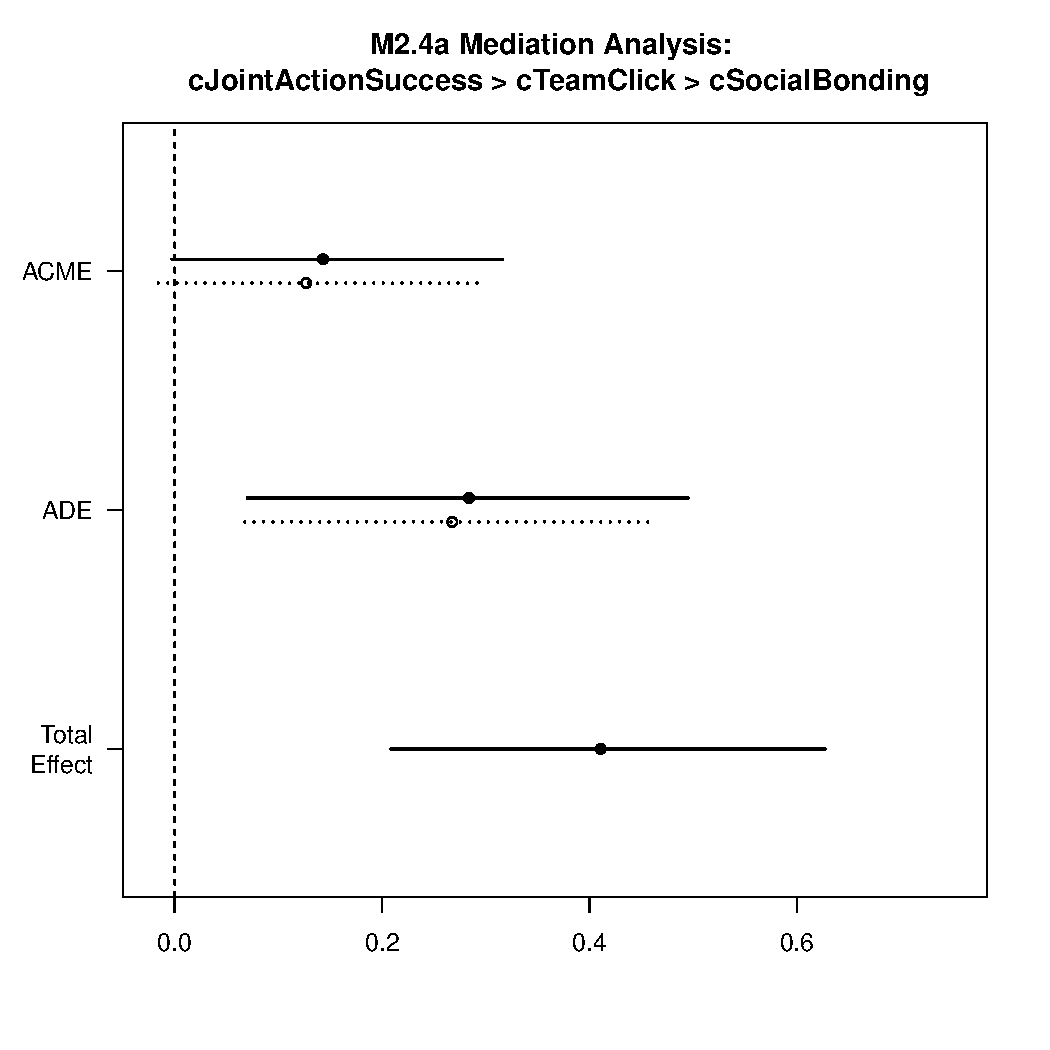
\includegraphics[scale=.5]{images/MLM24aMediationAnalysis.pdf}
      \caption{M24a Mediation Analysis}
      \label{fig:MLM24aMediationAnalysis}
    \end{figure}




\subsubsection{Prediction 4.b: Team Click mediates the relationship between Team Performance Vs Expectations and Social Bonding}

    \myparagraph{Post-Tournament}
  Results of the analyses above also demonstrate a significant positive relationship between Team Performance Vs Expectations and Team Click. The model generated for relationships between between Team Performance Vs Expectations and Social Bonding, however, was not robust to the demands of model assumptions.   Nonetheless, mediation analysis was used to test the possibility that Team Click mediated the effects of Team Performance Vs Expectations on Social Bonding.

  Results of the mediation analysis revealed significant average indirect effect of Team Performance Vs Expectations on Social Bonding attributable to Team Click, $\beta = .36, 95\% CI = .17 , .62, p < .0001$.  When controlling for the effect of Team Click on Social Bonding, the average direct effect between Team Performance Vs Expectations and Social Bonding was no longer significant, $\beta = -.07, 95\% CI = -.27 , .12, p = .84 $ (see Figure ~\ref{fig:MLM4bMediationAnalysis}). The total effect of the model was significant $\beta = .29, 95\% CI = .02 , .57, p = .04$.  This model, as with model 4.a above, indicated that Team Click fully mediated the relationship between Team Performance Vs Expectations and Social Bonding.


  Again, the results of this mediation model should be treated with caution, given the fact that the mediation model is composed of a non-robust statistical model (i.e., path ```'c'').

  \begin{figure}[htbp]
    \centering
    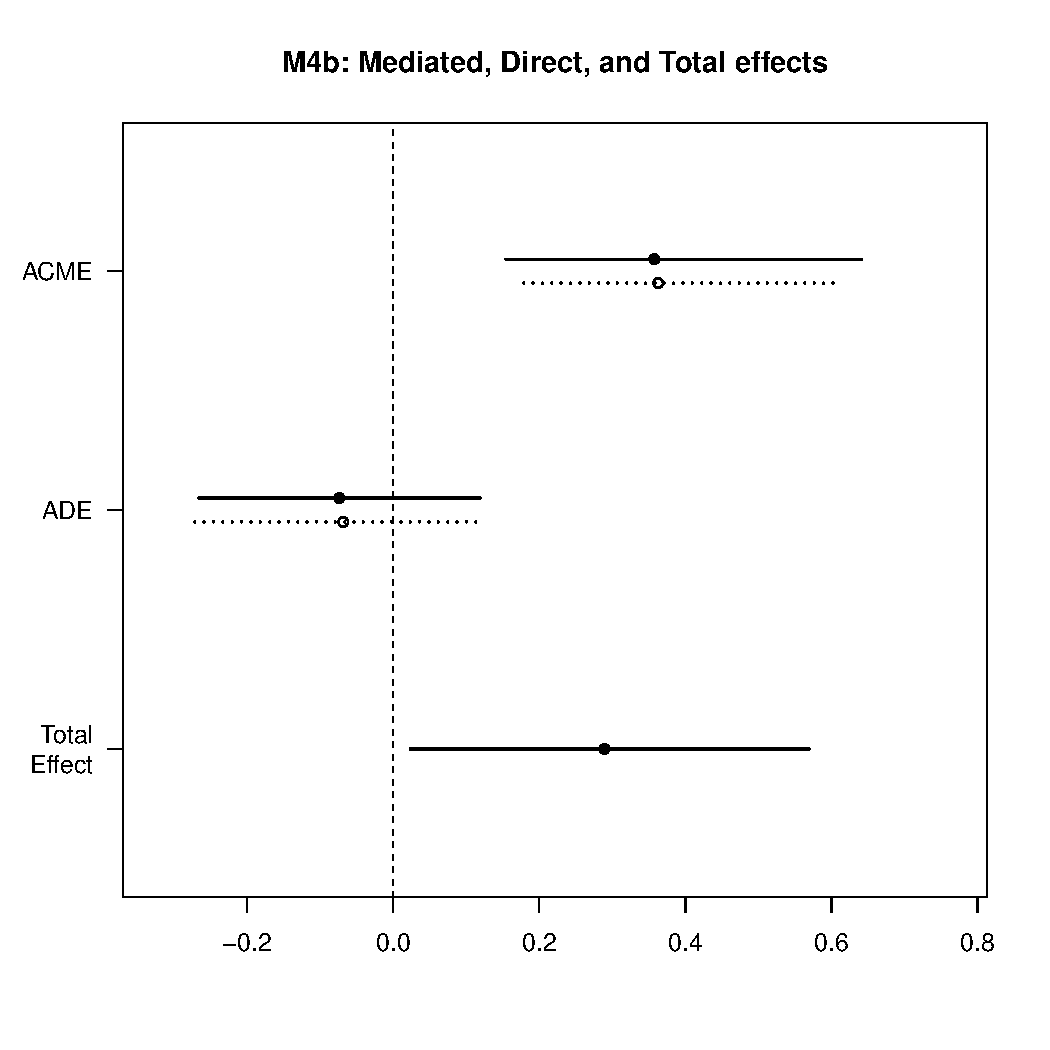
\includegraphics[scale = .5]{images/MLM4bMediationEffects.pdf}
    \caption{M4b Mediation Analysis}
    \label{fig:MLM4bMediationAnalysis}
  \end{figure}



  \myparagraph{Overall Tournament}

      %\subsubsection{3.4.b Social Bonding $\sim$ Team Performance Vs Expectations Tournament $\times$ Team Click Tournament}
In order to assess the possibility of a mediating effect of Team Click on the overall relationship between Team Performance Vs Expectations and Social Bonding, the interaction of Team Performance Vs Expectations and Team Click was added to a model as a fixed effect to see if an increase in social bonding associated with more positive violations of team performance expectations was heightened when feelings of team-click increased. The model revealed a significant negative interaction between Team Performance Vs Expectations and Team Click,  $\beta = -.26$ ($95\% CI =  -.32, -.20$), $SE = .03$, $t(321.2) = -8.46$, $p < .0001$, $marginal R^2 = .69$, $conditional R^2 = .74$.  Model residuals were non-normal ($W = .94, p < .00001$), owing to high kurtosis ($.39$) and negative skew ($-.88$) (see Appendix Figure ~\ref{fig:MLM32aAssumptions}).

A model in which the outcome variable was log transformed following exclusion of outliers provided the best adjustment: model residuals were normally distributed ($W = .99, p = .14$) and individual observations exerted low influence (Cook's Distances all < .10) (see Table ~\ref{MLM33ateamPerfBondingTournamentInteractionComparison} for full model comparison). The adjusted model revealed a significant positive interaction of Team Performance Vs Expectations and Team Click on Social Bonding, $\beta = -.06$ ($95\% CI =  .0004, .002$), $SE = .01$, $t(310.1) = -4.73$, $p < .001$, $marginal R^2 = .61$, $conditional R^2 = .65$. These results supported the prediction that feelings of team-click condition the relationship between perceptions of team performance (expectation violation, in this case) and feelings of social bonding.  Below, formal mediation analysis was conducted to further test this relationship.


       
% Table created by stargazer v.5.2 by Marek Hlavac, Harvard University. E-mail: hlavac at fas.harvard.edu
% Date and time: Thu, Sep 14, 2017 - 09:52:55
\begin{table}[!htbp] \centering 
  \caption{M3.3a socialBondingTournament ~ teamPerformanceExpectationsTournament*teamClickTournament} 
  \label{tab:MLM33ateamPerfBondingTournamentInteractionComparison} 
\scriptsize 
\begin{tabular}{@{\extracolsep{5pt}}lccc} 
\\[-1.8ex]\hline 
\hline \\[-1.8ex] 
 & \multicolumn{3}{c}{\textit{Dependent variable:}} \\ 
\cline{2-4} 
 & model & log-transformed & outliers+log-transformed \\ 
\\[-1.8ex] & (1) & (2) & (3)\\ 
\hline \\[-1.8ex] 
 (constant) & 0.45$^{**}$ & 1.69$^{***}$ & 1.62$^{***}$ \\ 
  & (0.16) & (0.04) & (0.06) \\ 
  & & & \\ 
 teamPerformanceExpectations & $-$0.0001 & $-$0.0003 & $-$0.001 \\ 
  & (0.002) & (0.0004) & (0.001) \\ 
  & & & \\ 
 indPerformanceExpectations & 1.02$^{***}$ & 0.22$^{***}$ & 0.11$^{**}$ \\ 
  & (0.06) & (0.01) & (0.04) \\ 
  & & & \\ 
 objectiveCompetence & 0.001 & 0.0003 & $-$0.0001 \\ 
  & (0.001) & (0.0004) & (0.001) \\ 
  & & & \\ 
 subjectiveCompetence & 0.01 & 0.01 & 0.01 \\ 
  & (0.04) & (0.01) & (0.01) \\ 
  & & & \\ 
 finalRank & 0.05 & 0.01 & 0.02 \\ 
  & (0.04) & (0.01) & (0.01) \\ 
  & & & \\ 
 minutesTotal & $-$0.03$^{*}$ & $-$0.01$^{*}$ & $-$0.01 \\ 
  & (0.02) & (0.004) & (0.01) \\ 
  & & & \\ 
 pointsTotal & $-$0.003 & $-$0.001 & $-$0.001 \\ 
  & (0.002) & (0.0005) & (0.001) \\ 
  & & & \\ 
 pointsTotal & 0.001 & 0.0001 & $-$0.001 \\ 
  & (0.003) & (0.001) & (0.001) \\ 
  & & & \\ 
 teamPerformanceExpectations:clickFactor3 & $-$0.01$^{***}$ & $-$0.002$^{***}$ & 0.002$^{*}$ \\ 
  & (0.001) & (0.0003) & (0.001) \\ 
  & & & \\ 
\hline \\[-1.8ex] 
Marginal R-squared & .68 & .28 & .23 \\ 
Conditional R-squared & .73 & .36 & .28 \\ 
Shapiro-Wilk Test (p-value) & .93($<$.00001) & .99(.02) & .99(.14) \\ 
Observations & 331 & 331 & 294 \\ 
Log Likelihood & $-$277.92 & 176.98 & 57.06 \\ 
Akaike Inf. Crit. & 589.83 & $-$319.96 & $-$80.12 \\ 
Bayesian Inf. Crit. & 654.47 & $-$255.32 & $-$17.50 \\ 
\hline 
\hline \\[-1.8ex] 
\textit{Note:}  & \multicolumn{3}{r}{$^{*}$p$<$0.05; $^{**}$p$<$0.01; $^{***}$p$<$0.001} \\ 
\end{tabular} 
\end{table} 


A mediation analysis was performed to formally test whether feelings of team click over the course of the Tournament mediated a direct relationship between team performance expectation violations and social bonding.  Results outlined above demonstrate Tournament-wide significant positive relationships between team performance expectation violations and feelings of team click, as well as team click and social bonding. Models also demonstrate a direct relationship between expectations around team performance and social bonding.  Available statistical software can only support a 2-level structure for multilevel mediation analysis. The third team-level random effect was therefore dropped from the model, while the model controlled for the random effect of individual across each of the four time points.

Results of the mediation analysis revealed that the average indirect effect of change in Team Performance Components on change in Social Bonding attributable to change in Team Click was highly significant albeit small, $\beta = .02, 95\% CI = .018 , .026, p < .001$.  When controlling for the effect of team click on Social Bonding, the average direct effect of Team Performance Vs Expectations and Social Bonding was also significant, $\beta = .01, 95\% CI = .001 , .017, p < .00001$.  The total effect of the meditation was also significant, $\beta = .03, 95\% CI = .027, .041, p < .0001$ (see Appendix Figure ~\ref{fig:MLM34aMediationAnalysis}).  These results suggest that Team Click \textit{partially} mediates the effect of Team Performance Vs Expectations and Social Bonding (average proportion mediated = .66 (.57, .77)).  This result should be treated with additional caution, as it did not account for team-level variation.

    \begin{figure}[htbp]
      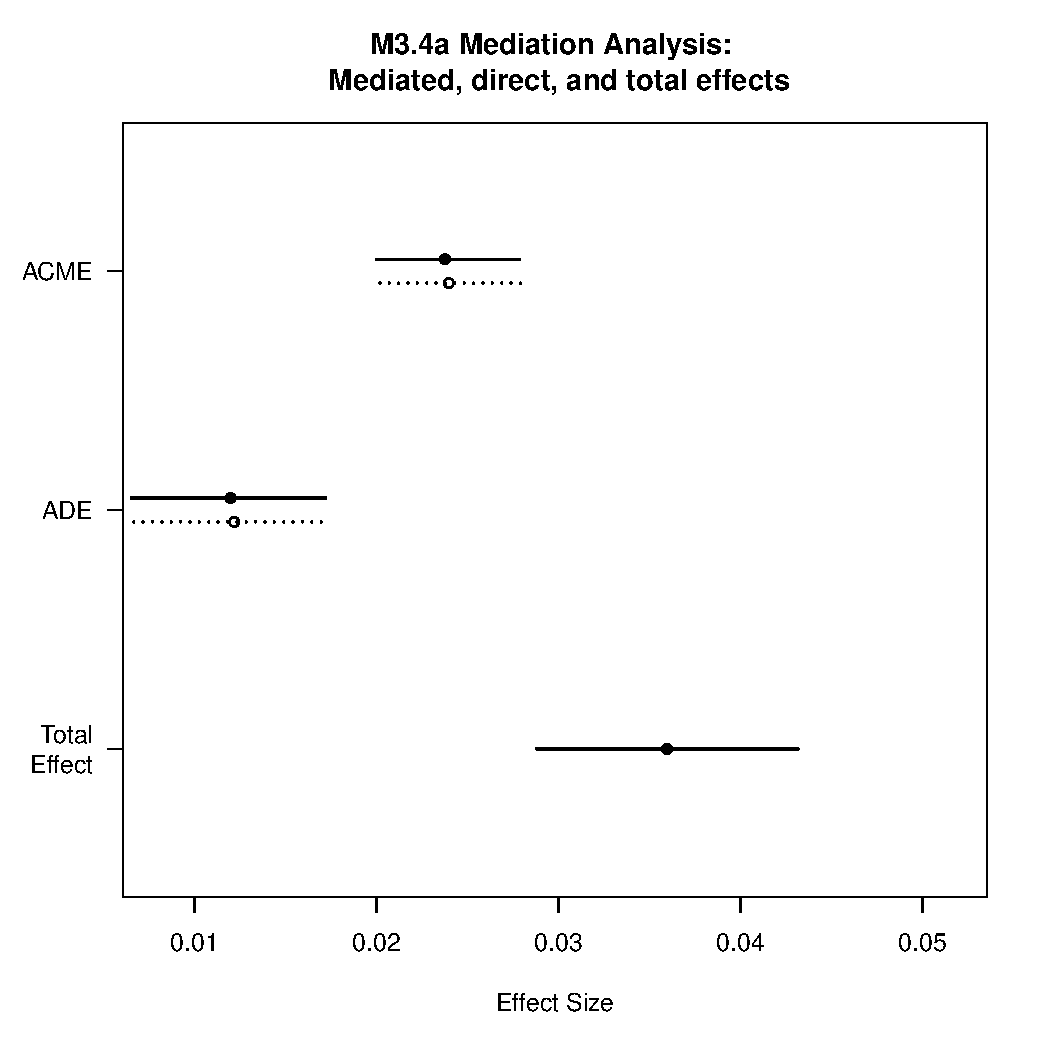
\includegraphics[scale=.5]{images/MLM34aMediationAnalysis.pdf}
      \caption{M3.4a Mediation Analysis}
      \label{fig:MLM34aMediationAnalysis}
    \end{figure}



\clearpage























\clearpage

\section{Discussion of Results}

Opening para:

Recap of method / approach


Main findings on the relationship between joint action, social bonding, and the mediating role of team click were the following:



21b: %The adjusted model also revealed a significant negative effect of violations of expectations around \textit{individual} performance on team click, $\beta = -.008 (95\% CI =  -.01, .001), SE = .004, t(91.79) = -2.28, p = .03$,  which could suggest that athletes who experienced more positive violations about their own performance did not feel the team click as strongly.


  The results presented above generally support the central hypothesis of this dissertation, namely that relationship the relationship between joint action and social bonding is mediated by the feeling of ``team click.''  Results of analyses concerning both the Post-Tournament survey and change between and Pre- and Post -Tournament surveys display a clear relationship between perceptions of Team Performance Components and Team Click, Team Click and Social Bonding, and a direct relationship between Team Performance Components and Social Bonding.  In the Post-Tournament analysis, Team Click fully mediates the relationship between Team Performance Components and Social Bonding. In the Pre-post analysis, Team Click partially mediates this relationship (this statistic was not significant, but was trending in the predicted direction, $p = .06$).

  Results of models designed to test the predicted relationships between Team Performance Vs Expectations, Team Click, and Social Bonding also provided support for some but not all predictions. A relationship was confirmed between team performance expectation violation and team click, but not between expectation violation and social bonding. In addition, the predicted interaction between Team Performance Components, Team Performance Vs Expectations, and Team Click was not significant, nor was the interaction between these same two predictor variables and social bonding.  Team click did not mediate the predicted relationship between violations of expectations around team performance and social bonding. The model of this direct relationship was not statistically robust using the data collected in this study.

  These results suggests that while expectation violation in joint action might be an important factor in generating feelings of team click, it might not be a strong enough mechanism to drive social bonding directly.  In contrast to the single-item measure of Team Performance Expectations, Team Performance Components is a factor made up of four items that require detailed reflection on the experience of four different aspects of team coordination.  This item may have more powerfully tapped into the implicit mechanisms involved in coordinated joint action, encouraging athletes to reflect on coordination with specific co-actors, and as such the opportunity to rehearse and reinforce feelings of trust, reliability, and cooperation \citep{Reddish2013a}.  It is also possible that expectation violation in joint action might not be immediately available to athlete reflection.
  As Frith and colleagues point out \textcite{Frith2007,Frith2010,Clark2013}, the generation of interoceptive predictive models for action implicates cognitive processes that exist largely below the surface of conscious awareness, and the relationship between these unconscious informational transfer in movement coordination and the small fraction of information that does make its way to consciousness in the form of higher order symbolic and linguistic representations is still not clearly understood \citep{Semin2008}. Team click might be supported by various subtle, implicit, and Pre-perceptual processes involved in ``active inference'' \citep{Schmidt2011}.

  Evidence presented here does however support the interpretations that perceptions of joint action success predict social bonding, mediated by the experience of ``team click.'' It was predicted that technical competence may condition the relationship between perceptions of joint action, team click, and social bonding, owing to the possibility that more expert athletes could be more likely experience less pronounced discrepancy between expected and actual performance \cite{Tomeo2012}.  In this specific study, there was no evidence that technical competence---objective competence (training age, years in team, age) and self-reported competence (ability versus teammates, Chinese opponents, or international professionals)---significantly influenced variables of interest.  It is possible, as noted above, that these measures failed to access the (largely Pre-perceptual) mechanisms of prediction error management hypothesised to underpin cognition and affective dispositions in joint action.  It is also possible that the nature of the intensity and consequentiality of the Tournament in which athletes were participating was high enough that no one---experts athletes included---was immune to the uncertainty and stress of this experience. Indeed, the ability of competitive group exercise contests to consistently arouse high levels of psychological stress and uncertainty could be an important reason for their cultural evolutionary success over recent centuries.

  In addition to technical competence of individual athletes, preexisting dispositional tendencies in dimensions of personality (e.g., extroversion, agreeableness) and physical endowment could impact on processes of social bonding \citep{Marsh2009,VonRueden2015}.   It has been documented that personality types correspond with basal tendencies for movement and movement coordination. In a joint action task involving two people of different heights moving wooden planks of different lengths, for example, Richardson and colleagues \textcite{Richardson2007} found that individuals’ levels of agreeableness and extroversion were positively correlated with the level of persistence of cooperation (hyteresis).  In particular, in the condition in which wooden planks increased in length (therefore increasing in demand for cooperative action), the degree of cooperation was positively correlated with the taller of the pair’s extroversion; the degree of cooperation in the random condition (where planks were received in no ordinal sequence of sizing) was correlated with the agreeableness of the shorter (i.e., more constraining) of the individuals.  I used the personality data collected in the Pre-Tournament survey to test the relationship between personality types and team click. Interestingly, none of the big five personality types (extraversion, agreeableness, openness, conscientiousness, and neuroticism) significantly predicted feelings of team click in the Post-Tournament survey.

  The impact of inter-individual psychophysiological variation on joint action can also be seen in the case of social dysfunctions such as autism spectrum disorder \citep{Isenhower2012} and schizophrenia \citep{Varlet2012}.  Generally speaking,  while autism spectrum disorder appears to be associated with deficits in anticipatory timing adjustments in intra- and inter-individual coordination of physical movement \citep{Martineau2010}, schizophrenia appears linked to a lack of prediction error management, due to failure in the neurological mechanisms through which predictions about the consequences of an action are derived \citep{Frith2000}.  Delusions of control owing to misattribution of agency are well-documented in schizophrenic patients---either delusions of self-control over external actions and events, or, alternatively, delusions involving the control of others over the individual (in the case of split personality and associated hallucinations) \citep{Frith2007}. It is quite possible that the experience of ``team click'' is an analogue, albeit a much more socially functional one, to the pathological over-activity of agency-attribution mechanisms observed in schizophrenic patients.  The question of individual variation in sociability and movement tendencies should be further assessed in future studies.

  The fact that the hypothesised mechanisms of joint action and social bonding have been shown to exist Pre-declaratively and predominantly below the surface of conscious experience presents a methodological challenge for psychological research which relies heavily on self-report.  Further exploring the relationship between Pre-perceptual regulatory mechanisms of joint action and their psychosocial effects will require the use of other methods of data collection and analysis in order to triangulate the reliability of self-report data \citep{Newell2014}.  In this specific example, video footage showing athlete performance and coordination could be assessed using already established methods of motion capture and analysis to provide pseudo-objective measures of interpersonal and team-level synchrony in joint action \citep[e.g.][]{Passos2011}.
  Importantly, video footage analysis allows for the testing between different proposed mechanisms associated with joint action and social bonding,  For example, motion capture from video footage allows for measuring synchrony between co-actors could using both traditional methods of dimension reduction and principal component analysis \citep[see for example][]{Riley2011} as well as emerging methods borrowed from dynamic systems theory including fractal-like 1/f scaling (``pink noise'') \citep[see for example][]{Holden2013}. It is quite possible that these different measurements of synchrony could access different psychophysiological dimensions of the relationship between joint action and social bonding.  Other physiological markers of social interaction such as heart rate variability \citep{Konvalinka2011,Fischer2014a} and pain threshold \citep{Cohen2009,Tarr2015}) are beginning to be developed and tested in both experimental and real-world settings.
  These novel methodological approaches help complement existing behavioural measures, such as such as economic games \citep{Xygalatas2013} and spontaneous helping tasks \citep{Kirschner2010}, designed to access psychological mechanisms related to social bonding and cooperation.
  Together, these measures could then be compared to self-report measures derived from athlete self-report to more fully understand the ways in which component mechanisms and system dynamics of joint action generate social cohesion \citep{Marsh2009}.

  In sum, the results reported in this study provide novel evidence that feelings of team click mediate a relationship between perceived joint action success and social bonding, substantiating the claim that under certain circumstances joint action and interpersonal coordination processes can generate feelings of social connection \citep{Marsh2009}. Relationships between expectation violation, team click, and social bonding
  also confirmed, but these models are less robust, and should be treated with caution. All reported results hold when statistically controlling for measures relating to individual performance, objective competence, and actual Tournament performance outcomes in the Tournament, including Tournament rank, points scored, minutes played, and so on.  Of course, the uncontrolled and \textit{in-situ} design of this study means that results are correlational, and as such the predictions of this dissertation, only partially confirmed in this study, require further attention via a controlled experimental design.  An experiment in which joint action success and expectation violation were manipulated, and explicit feedback around performance was eliminated, could allow for the assessment of the role of the cognitive processes of movement coordination in joint action in generating team click and social bonding.  In addition, a controlled experiment offers the opportunity to utilise other measurements of synchrony, such as those derived from motion capture from video recordings.


%    [ ] what inferences can we make from these results?
%    [ ] How does it relate to other literature?
%    [ ] limitations
%    [ ] future work —> experiment (takes away explicit feedback)
%    [ ]  "Conclude the general discussion with a strong paragraph stating the main point or points again, in somewhat different terms-if possible-than used before.”
                                                \end{CJK}{UTF8}{gbsn}
